\chapter{Grundlagen}
\label{sec:fundamentals}
\todo[color=blue!40]{Feedback zu Struktur des Literaturkapitels}\section{Software Qualitätssicherung}
\subsection{Motivation und Relevanz}

\todo{Evt. einleitende Worte...}
Der Funktionsumfang von Software stieg in den letzten fünzig Jahren enorm. Gleichzeitig bietet die Geschichte der Informatik viele Beispiele, die für die Notwendigkeit von Qualitätssicherung in der Softwareentwicklung sprechen. Ein sehr bildhaftes Beispiel der Folgen von fehlerhafter Software, ist die Selbstzerstörung der Ariane 5 Rakete im Jahr 1996 \cite{giese_warum_2002}. Das Trägheitsnavigationssystem wandelte eine 64-bit-Gleitkommazahl in eine Ganzzahl. Dieser Programmteil wurde schon in der Ariane 4 verwendet, nur war diese weitaus schubschwächer und der betroffene Sensor erzeugte viel kleinere Ergebnisse. Nur 36 Sekunden nach Start des Erstfluges, setzte also ein klassischer Überlauf ein und die Rakete aktivierte ihren Selbstzerstörungsmechanismus.
Ähnliches passierte bei der Raumsonde Mars Obiter der NASA. Diese war am 24. September 1999 gestartet und hätte 220 Millionen Kilometer später auf dem roten Planeten landen sollen. Kurz vor der Landung ging der Kontakt verloren, die Sonde zerschellte an der Oberfläche des Planeten. In diesem Fall war es kein Überlauf sondern ein Fehler bei den Maßeinheiten die den Steuerungsschub kontrollierten. Die Entwickler der NASA erwarteten in ihrem Code Zahlen in Form von Newton, während der Hersteller Lockheed Martin angloamerikanische Pfund lieferte.Durch Zufall fiel der Fehler während des gesamten Flugs nicht auf. \cite{thaller_software-test:_2002}
In keinem der beiden Vorfälle kamen Menschen zu Schaden, trotzdem waren die finanziellen Verluste enorm. Natürlich war die Komplexität dieser NASA-Projekte sehr hoch und wahrscheinlich nicht repräsentativ für Software die am Markt erhältlich ist, trotzdem wären beide Fehler durch Testing vermeidbar gewesen. Im Fall der Ariane 5 hätte es ausgereicht die Schnittstelle zum Steuercomputer mit Extremwerten zu testen. Man wäre schnell auf den Überlauf gestoßen und hätte die Umrechnung anpassen können. Auch Mars Orbiter hätte durch ausführliches Schnittstellen-Testing auf Basis von Verträgen, welche die beteiligten Software-Teams untereinander ausmachen, gerettet werden können.

\subsubsection{Der Zwang zu qualitativem Wachstum}
Die Qualität von Software erhöhte sich geschichtlich nicht im selben Maße wie ihre Funktionalität. Der Drang nach Wachstum bei modernen Programmen negiert die Erfolge die Unternehmen durch erhöhte Anstrengungen in der Qualitätssicherung feiern könnten. Die Zahl der Fehler wird weitläufig gesenkt,  gleichzeitig nimmt der Funktionsumfang der Programme massiv zu. Dieser Umstand rührt daher, dass ständig neue Käuferschichten gewonnen werden müssen, die wiederum neue Features fordern.
Software dringt in Gebiete vor die von analoger Technik dominiert wurden. Aeronautik, Medizin und Finanzwesen verlangen nach großen Programmpaketen, die potenziell viele Fehlerquellen mit weichreichenden Folgen enthalten.

\subsubsection{Komplexe Systeme führen zu Fehlern}
Von der Programmierung in Hochsprachen bis zur Ausführung auf der Hardware müssen unzählige Schichten korrekt ineinander greifen um das gewünschte Ergebnis hervorzubringen. 
Daher gilt:

\begin{quote}
Komplexe Systeme analytisch in begrenzer Zeit nur unvollständig erfassbar. Fehler sind damit zwangsläufig die Folge. \cite{vigenschow_objektorientiertes_2004}
\end{quote}

Gründe wieso Fehler auftreten sind mannigfaltig. Aus menschlicher Sicht können Fehler auf drei Ebenen auftreten: \cite{vigenschow_objektorientiertes_2004}

\paragraph{Kommunikation}
Jegliche Art von Kommunikation ist Transformation \cite{shannon_mathematische_1976}. Dabei passieren diese Transformationen nicht nur bei der Kommunikation zwischen zwei Menschen sondern auch bei der Transformation von Sprache in Verständnis. Naturgemäß bleibt bei diesen Transformationen Informationsgehalt verloren, abhängig von verschiedenen Rahmenbedingungen manchmal sogar sehr viel, beispielsweise wenn Information in einer Sprache übermittelt wird, welche nicht die Muttersprache von beiden Kommunikationspartnern ist.
Im technischen Umfeld gibt es darum viele Standardbegriffe, die möglichst genau definiert sind. So soll der Informationsverlust eingeschränkt werden.
Weiters spielt sich ein nicht unerheblicher Teil der Kommunikation auf unterbewusster Ebene ab.

\paragraph{Fachlichkeit}
Kunden oder Auftraggeber sind naturgemäß Experten auf ihrem Gebiet. Sie wollen Software um ihre fachlichen Ziele effektiver verfolgen zu können. Dem Software-Entwickler fehlt dieses Fachwissen. Dem Entwickler fehlt dieses Fachwissen oft.
Der Kunde hat sehr detaillierte Vorstellungen der Software, ihm fehlt aber die Fähigkeit auf technischer und fachlicher Ebene zu abstrahieren. Dies ist eine der Hauptaufgaben des Requirements-Engineer. Genau an dieser Stelle ist die Gefahr groß, dass durch fehlendes fachliches Wissen wichtige Zusammenhänge übersehen werden oder unwichtigen Details zu viel Aufmerksamkeit geschenkt wird.
Außerdem sind die technischen Möglichkeiten nur eingeschränkt für den Kunden fassbar. Gerade Aufwandsschätzungen sind für Entwickler schon schwierig Das hat zur Folge, dass die Entwickler oft Alternativen anbieten müssen welche möglicherweise nicht den exakten Anforderungen entsprechen.

\paragraph{Komplexität}
Die Komplexität der Problemstellung bestimmt über Machbarkeit und Fehlerpotenzial. Seit Anbeginn der Informatik wird versucht Komplexität auf ein überschaubares Maß herunterzubrechen. Sei es durch Zerlegung in möglichst kleine Aufgaben, visuelle Darstellungsformen oder Abstraktion zu bekannten Programmiermustern.
Komplexität wird dadurch aber niemals vermindert, sondern nur versteckt bzw. anschaulicher gemacht.


\subsection{Softwarequlität und Standards}
\label{sec:quality}
Der Begriff Qualität kann auf vielfältige Art und Weise definiert werden. Jeder Mensch hat ein gewisses intuitives Verständnis dafür. Bezogen auf verschiedene Anwendungsfelder assoziiert ein Jeder andere Merkmale eines Objekts mit Qualität.

\begin{quote}
Entscheidend ist, was die Anspruchsteller vor dem Hintergrund ihrer Anforderungen wahrnehmen und für wichtig halten. Während die rational bedingte Sachqualität mit naturwissenschaftlich-technischen Methoden messbar ist, bereitet die reproduzierbare Messung der Anmutungsqualität Probleme.\cite{markgraf_definition_2015}
\end{quote}

Im Kontext der Software-Entwicklung verbinden Entwickler und Projektleiter mit dem Begriff der Qualität verschiedene Inhalte.\cite{hoffmann_software-qualitat_2013} Aus diesem Grund wurde bereits mehrfach versucht, eine einheitliche Definition für den Begriff Qualität zu finden. Die, inzwischen überholte DIN-ISO-Norm 9126 \footnote{ISO 9126: Software Quality \url{http://www.iso.org/iso/catalogue_detail.htm?csnumber=22749}} definiert Softwarequalität wie folgt:

\begin{quote}
Software-Qualität ist die Gesamtheit der Merkmale und Merkmalswerte eines Software-Produkts, die sich auf dessen Eignung beziehen, festgelegte Erfordernisse zu erfüllen.
\end{quote}

Diese Definition unterstreicht, dass der Begriff Software-Qualität eine multikausale Größe beschreibt.\cite{hoffmann_software-qualitat_2013} Vor dem Hintergrund, des sich rasant entwickelnden Gebiets der Software-Entwicklung, gibt es nun eine stark überarbeitete Version dieser ISO-Norm. Die Normenreihe ISO/IEC 25000 umfasst nun über ein dutzend Standards die sich sehr detailliert mit der Thematik auseinandersetzen. Dazu zählen unter anderem Leitfäden zu Planung und Management, Metriken zur Qualitätsmessung und Anforderungen an Datenqualität. Im Wesentlichen definiert ISO/IEC 25010 \footnote{ISO/IEC 25010: Systems and Software Quality Requirements and Evaluation (SQuaRE) \url{http://www.iso.org/iso/home/store/catalogue_ics/catalogue_detail_ics.htm?csnumber=35733}} eine Reihe vielschichtiger Kriterien, welche als Bausteine der Software-Qualität verstanden werden können.

\paragraph{Funktionalität (Functionality, Capability)} Dieses Qualitätsmerkmal beschreibt, in welchem Maß ein Software-System den ihm zugeschriebenen Funktionsumfang tatsächlich erfüllt. Funktionale Fehler entstehen aus den verschiedensten Umständen. Möglich sind Fehler die passieren wenn Anforderungen auf eine nicht beabsichtigte Art und Weise implementiert werden. Andererseits lassen sich funktionale Fehler auch oft auf unvollständige oder nicht vorhandene Spezifikationen zurückführen. Äußere Faktoren wie Zeitmangel oder zwischenmenschliche Unstimmigkeiten haben einen besonders negativen Einfluss auf die häufigste Art von funktionalen Fehlern: Klassische Implementierungsfehler (sogenannte ``bugs''). Diese sind auch das Hauptaugenmerk der Methoden und Techniken der Software-Qualitätssicherung. Weil funktionale Fehler so allgegenwärtig sind, wird der Begriff der Software-Qualität häufig auf dieses eine Kriterium reduziert wahrgenommen.

\paragraph{Laufzeit (Performance)} Jedes Software-System unterliegt gewissen Laufzeitanforderungen. Oft wird diesen aber bei der Formulierung der Anforderungen weniger Beachtung, als funktionalen Anforderungen, geschenkt. Laufzeitanforderungen können bei Nichtbeachtung sehr lange Zeit unentdeckt bleiben, sich dann aber zu ernstzunehmenden Problemen entwickeln.\\
Im Bereich der Echtzeitsysteme unterliegen alle Operationen Zeitanforderungen, die entweder im statistischen Mittel (weiche Echtzeit) oder in jedem Einzelfall (harte Echtzeit) zwingend erfüllt werden müssen. \cite{hoffmann_software-qualitat_2013}

\paragraph{Zuverlässigkeit (Reliability)} In sicherheitskritischen Anwendungen kann sich ein Systemversagen direkt auf die Unversehrtheit der beteiligten Personen auswirken. Zuverlässigkeit ist aber eng mit anderen Kriterien gekoppelt und kann (und soll) nicht als einzelnes Ziel erreicht werden.

\paragraph{Wartbarkeit (Maintainability)} Wartbarkeit und Langlebigkeit sind zentrale Qualitätsmerkmale moderner Software-Systeme. \cite{rombach_design_2009} In vielen Fällen hört die Projektplanung bei der Inbetriebnahme der Applikation auf und ignoriert die Notwendigkeit, nachträglich Anpassungen zu machen und Fehler zu beheben.

\paragraph{Transparenz (Transparency)} Der Grad der Transparenz beschreibt wie die nach außen sichtbare Funktionalität, intern umgesetzt wurde. Eine zentrale Fragestellung ist: ``Lässt sich durch Betrachtung des Programms von außen (aus Blackbox-Sicht \todo{Ref zu Blackbox-Beschreibung}) auf die internen Vorgänge des Codes schließen?''. Wenn diese Durchsichtigkeit gegeben ist, spricht man von hoher Transparenz. Ein Programm kann geforderte Funktionalität aber auf unendlich viele Art und Weisen bedienen (man denke an Problemstellungen der theoretischen Informatik, wie die Church-Turing These\footnote{Die Church-Turing These trifft Aussagen über die Mächtigkeit von Programmiersprachen. \cite{hoffmann_theoretische_2011} Da sich unendlich viele Programmiersprachen definieren lassen, kann man darauf schließen, dass sich ein Programm auf unendlich viele Art und Weisen schreiben lässt.}) Die Transparenz trifft daher keine Aussage über die Richtigkeit des Programms. Statistisch gesehen nimmt die Transparenz eines Software-Systems im Zuge seiner Weiterentwicklung kontinuierlich ab.\cite{hoffmann_software-qualitat_2013} Man sprich davon, dass Software altert oder von Software-Entropie. Der Grad der Transparenz ist daher eng mit \textit{Wartbarkeit} und \textit{Testbarkeit} gekoppelt. 

\paragraph{Übertragbarkeit (Portability)} Übertragbarkeit beschreibt die Einfachheit bestehende Software auf andere Umgebungen oder Plattformen zu übertragen. Dabei ist Ausschlaggebend wieviel Aufwände in die Umstrukturierung und Umprogrammierung des Software-Systems fließen müssen. Wie so oft, müssen bei der Betrachtung von Übertragbarkeit, zum Zeitpunkt des Entwurfs der Software, Kompromisse eingegangen werden. Software wird vielfach nur für wenige geplante Zielplattformen designed und entwickelt, muss dann im weiteren Verlauf aber für andere Plattformen erweitert werden.

\paragraph{Testbarkeit (Testability)} Die Testbarkeit beschreibt wie gut oder schlecht ein Software-System testbar ist. Fehler sollen zeitnah gefunden und behebbar sein (Wartbarkeit). Testbarkeit wird schon zum Entwurfszeitpunkt bestimmt (design for test). Es geht darum, ob ein Programm geeignete Schnittstellen für das Testing bietet (sozusagen Zugriff auf seine Interna zulässt). Gängige Beispiele sind Logging-Funktionalitäten oder Schnittstellen die Benutzerinteraktionen simulieren.

Die Kriterien \textit{Funktionalität, Laufzeit, Zuverlässigkeit} und \textit{Benutzbarkeit} sind unmittelbar nach außen sichtbar und repräsentieren die Qualiätssicht des Benutzers. Folglich beeinflussen diese Kriterien die initiale Kaufentscheidung massiv. Die Kriterien \textit{Transparenz, Übertragbarkeit, Wartbarkeit} und \textit{Testbarkeit} offenbaren sich dem Benutzer üblicherweise viel später. Sie entscheiden über den langfristigen Erfolg und wie sich ein Software-Produkt am Markt hält.

\subsubsection{Zusammenhänge und Kompromisse} 
Nach Evaluation all dieser Kriterien kann eine Aussage über die Qualität von Software getroffen werden. Sie beeinflussen sich gegenseitig. Am Beispiel von \textit{Laufzeit} und \textit{Übertragbarkeit} lassen sich diese Zusammenhänge gut erkennen. Hochperfomante Software-Systeme nutzen viele Spezialitäten der verwendeten Programmiersprache und der Plattform auf dem sie betrieben werden. Wenn aus fundamentalen Bausteinen wie Architektur und Design keine weiteren Leistungssteigerungen gewonnen werden können, muss auf solche ``Adaptions-Tricks'' zurückgegriffen werden um den entscheidenden Vorsprung gegenüber Konkurrenzprodukten zu gewinnen. Die Übertragbarkeit eines Systems definiert sich aber wesentlich durch die ausschließliche Verwendungen von Konstrukten die in möglichst vielen Umgebungen verfügbar ist. Plattformabhängigkeiten müssten daher wieder generalisiert werden, was mit Aufwänden verbunden ist.\\
Deshalb ist es auch nicht möglich, ein Software-System zu entwickeln, das alle genannten Qualitätskriterien gleichermaßen erfüllt. Solche Aussagen sind aber nicht nur auf Software zu beschränken. Es handelt sich um sehr allgemeine Gesetzmäßigkeiten, die bereits in der Forschung zur klassischen Evolutionstheorie aufgedeckt wurden.\cite{hoffmann_software-qualitat_2013} Dies erklärt auch, weshalb viele dieser Zusammenänge intuitiv Sinn machen. Nicht alle Qualitätskriterien beeinflussen gleich viele andere Kriterien. Auch positive Effekte sind erkennbar. Eine hohe \textit{Testbarkeit} beeinflusst \textit{Zuverlässigkeit} positiv. Abbildung \ref{fig:korrelationsmatrix} zeigt die Vereinbarkeit/Unvereinbarkeit der Qualitätskriterien, die in der Softwareentwicklung eine Rolle spielen. Es wird deutlich welche Qualitäten kompromitiert werden müssen wenn andere im Projekt einen höheren Stellenwert haben. Gleichzeitig wird verdeutlicht, dass verschiedene Kriterien positive Auswirkungen aufeinander haben.

\begin{figure}[h] 
  \centering
     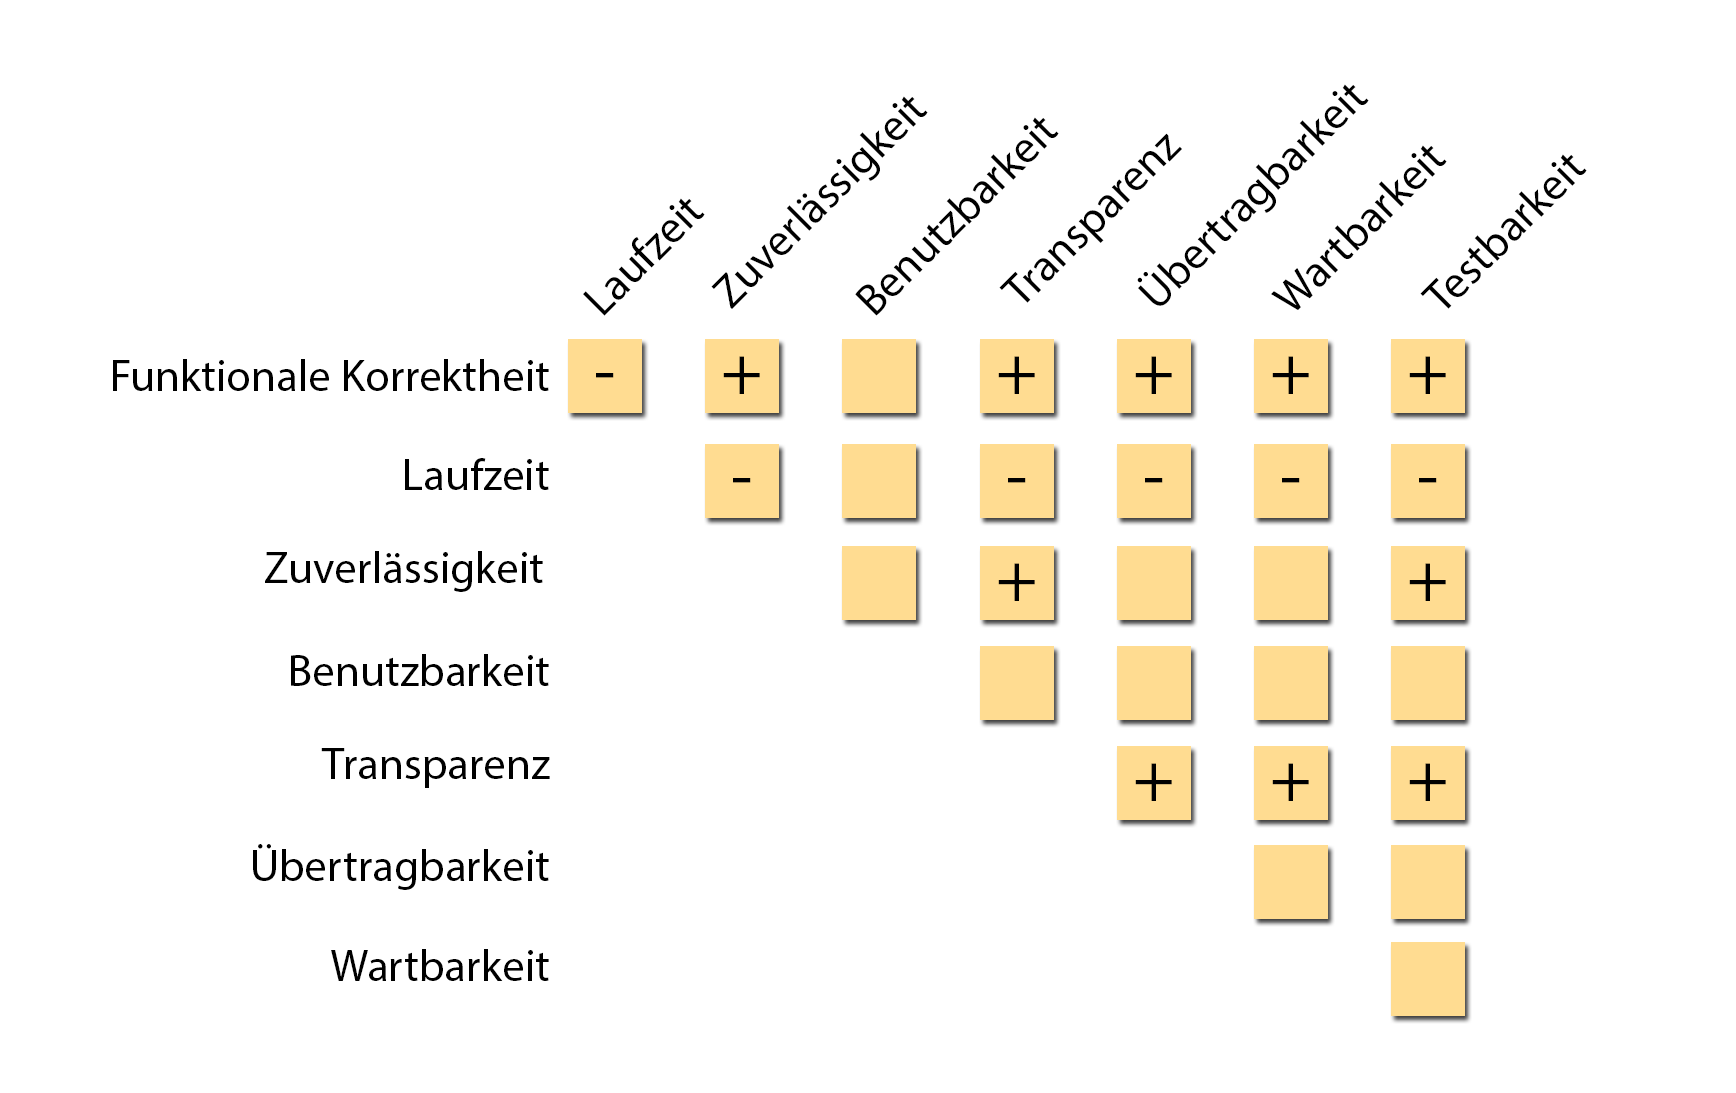
\includegraphics[width=0.9\textwidth]{figures/korrelationsmatrix.png}
  \caption{Die Korrelationsmatrix über die genannten Qualitätskriterien\cite{hoffmann_software-qualitat_2013}}
  \label{fig:korrelationsmatrix}
\end{figure}

Aus dem Projektmanagement ist das magische Dreieck bekannt (siehe Abbildung \ref{fig:magic_triangle}), das sich unmittelbar aus den eben genannten Korrelationen ableiten lässt. Die äußeren Eckpunkte des Dreiecks geben an, in welchem Maß die Parameter \textit{Zeit}, \textit{Kosten} und \textit{Qualität} erfüllt sind. Der Flächeninhalt des Dreiecks soll konstant sein, was veranschaulicht, dass jede Erhöhung eines Parameters die anderen beiden beeinflusst. Dieses Dreieck wird nicht nur durch die gewählten Entwicklungstechnologien und Requirements beeinflusst, sondern auch durch die Teststrategie. Welche Testmethoden und Werkzeuge gewählt werden, beeinflusst alle drei Parameter.

\begin{figure}[h] 
  \centering
     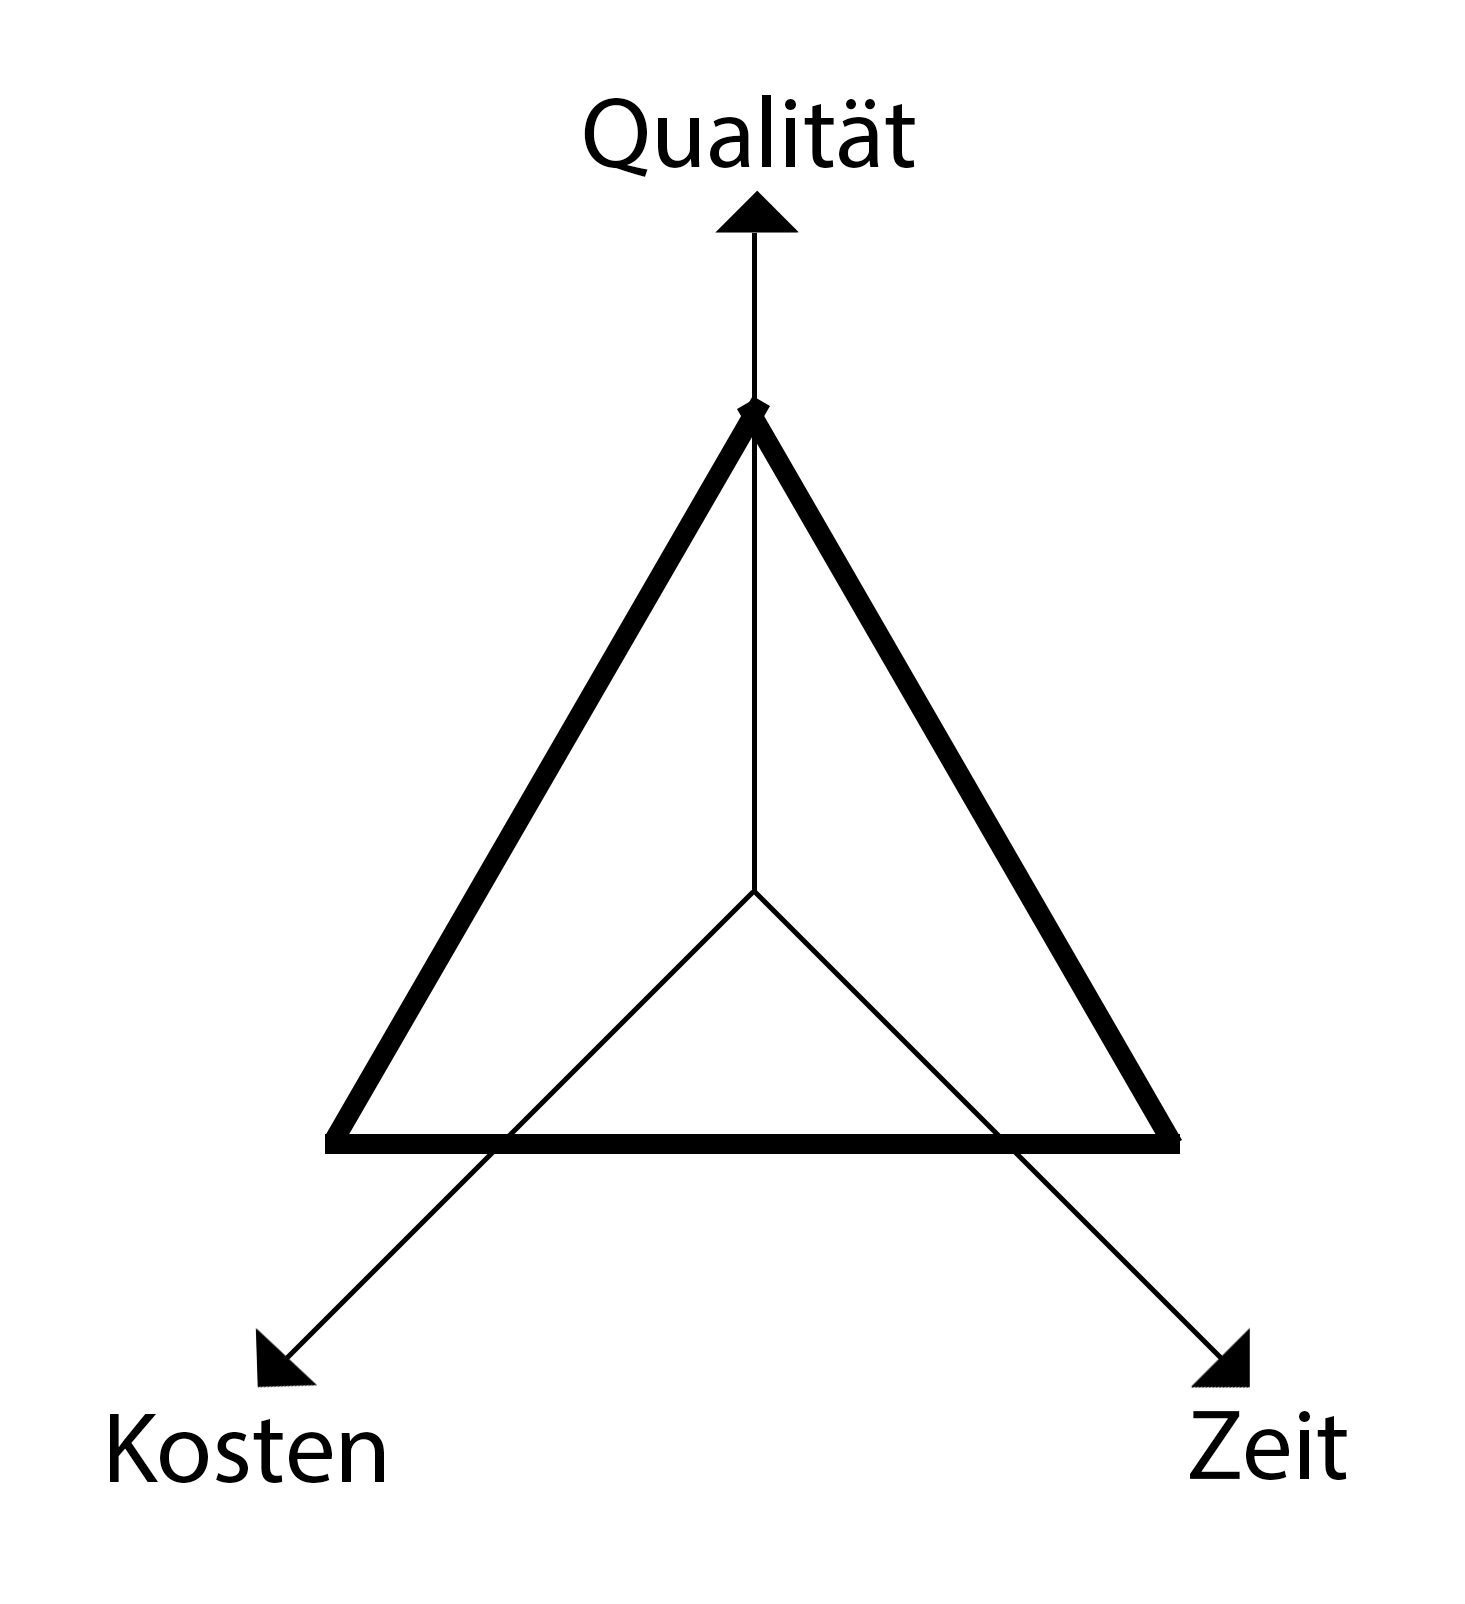
\includegraphics[width=0.7\textwidth]{figures/magic_triangle.png}
  \caption{Dieses Dreieck veranschaulicht wie sich die Qualitätsparameter Qualität, Zeit und Kosten gegenseitig beeinflussen. Die Fläche des Dreiecks bleibt fixiert, während die Seitenlängen verändert werden.}
  \label{fig:magic_triangle}
\end{figure}


\subsection{Testprozess}

\subsection{Teststufen}
Jedes Softwareentwicklungsvorhaben sollte nach einem genau definierten Vorgehensmodell spezifiziert, entwickelt, gewartet und getestet werden\cite{spillner_basiswissen_2012}. Nach wie vor orientieren sich moderne Softwareprojekte am sogenannten V-Modell\cite{boehm_verifying_1984} oder an einer davon abgewandelten Form. Der Grundgedanke hinter dem V-Modell ist es eine Parallelität und Gleichberechtigtkeit zwischen Entwicklungs- und Testtätigkeiten zu schaffen. Dies impliziert unmittelbar, dass die Teststrategie an die Entwicklungsstrategie angepasst werden muss, oder umgekehrt.\\
\todo{Abbildung zu V-Modell siehe Basiswissen SWT Seite 38} Abbildung XY zeigt ein klassisches V-Modell und dessen Komponenten. Es ist sofort erkenntlich, dass die Aktivitäten auf der linken Seite eng an das Wasserfallmodell angelehnt sind.
\begin{itemize}
\item \textbf{Anforderungsdefinition} Die Anforderungen des Kunden werden erhoben und möglichst präzise spezifiziert.
\item \textbf{Funktionaler Systementwurf} Auch Pflichtenheft genannt. Die Anforderungen werden auf Funktionen und Dialogabläufe des neuen Systems abgebildet\cite{spillner_basiswissen_2012}
\item \textbf{Technischer Systementwurf} Bezieht sich auf die technische Realisierung des Systems. Architektur und fundamentale Technologien werden hier bestimmt.
\item \textbf{Komponentenspezifikation} Für jede zuvor definierte Komponente wird eine Spezifikation geschrieben. Diese enthält den inneren Aufbau, die Schnittstellen nach Außen und die Abhängigkeiten zu anderen Komponenten.
\item \textbf{Programmierung} Die Implementierung jeder Komponente und die Verbindung all dieser zu einem funktionsfähigen Gesamten.
\end{itemize}

Parallel zu jeder dieser Tätigkeiten besteht eine Testaktivität, die die Implementierung gegen die ursprüngliche Spezifikation validiert. Ein Tester bewertet ob das System bzw. die Komponente für die definierten Use-Cases einsetzbar ist. Untersucht wird, ob das Produkt im Kontext der beabsichtigten Produktnutzung sinnvoll ist\cite{spillner_basiswissen_2012}.\\
Außerdem erfordert das V-Modell auch verifizierende Prüfungen, die auf einzelne Phasen bezogen das Ergebniss ebendieser prüft und mit der ursprünglichen Spezifikation vergleicht.\\
Die folgenden Teststufen sollen eine möglichst hohe Softwarequalität sicherstellen und nehmen oft Bezug auf die in Abschnitt \ref{sec:quality} genannten Qualitätsziele.

\subsubsection{Komponententest}
In der ersten Teststufe des V-Modells werden die kleinsten Softwarebausteine einer systematischen Prüfung unterzogen. Abhängig von der verwendeten Programmiersprache sind diese kleinsten Bausteine Module oder Klassen, dementsprechend spricht man dann von Modul- bzw. Unit-Tests.\\
Komponententests zeichnen sich außerdem durch die zeitliche Nähe zur Programmierung aus. Sie werden üblicherweise direkt vor oder nach der Programmierung einer Komponente verfasst. Der Komponententest unterscheidet sich vom Integrationstest durch seine Isolation. Das bedeutet die Funktionalität jeder Komponente wird ohne Ein- oder Zugriffe anderer Komponenten getestet. Dies hat den Zweck, dass ein Fehlverhalten auf die Komponente selbst zurückgeführt werden kann und fehlerhafte Einwirkung von außen ausgeschlossen werden kann.\\
Der Komponententest gehört zur Kategorie der White-Box Tests. Der Tester muss Zugriff auf den Quellcode des Programms haben, weil die kleinsten Softwarebausteine keine Schnittstelle nach außen haben. Deshalb liegt es nahe, dass Komponententests von den Entwicklern selbst geschrieben werden (was auch in den meisten Softwareprojekten so gehandhabt wird).  

\paragraph{Testziele auf Komponententestebene}
Oberstes Ziel der Komponententests ist die Sicherstellung, dass jede Komponente ihre spezifizierte Funktionalität fehlerfrei erfüllt. Funktionalität ist dabei gleichbedeutend mit dem Ein-/Ausgabe-Verhalten des Testobjekts\cite{spillner_basiswissen_2012}.\\

\subparagraph{Robustheit} Weil Komponenten in modernen Softwaresystemen mit einer Vielzahl von anderen Komponenten innerhalb des Systems und sogar außerhalb des Systems arbeiten müssen, muss sichergestellt werden, dass Fehlersituationen abgefangen und sinnvoll kommuniziert werden. Diese Eigenschaft wird Robustheit genannt. Um Robustheit bewerten zu können werden Eingabedaten gemacht, die bewusst zu einem Fehlverhalten führen (Negativtests). Die Ausgabewerte werden dann auf angemessene Ausnahmebehandlung geprüft (\textit{exception handling}). Erstens ist wichtig, dass überhaupt Ausnahmen gemeldet werden und ein Fehlverhalten nicht stillschweigend weitergereicht wird. Dieser Umstand kann weitreichende Folgen haben und zu schwer nachvollziehbaren Fehlern führen. Zweitens wird die Qualität der Ausnahmebehandlung bewertet. Diese muss möglichst aussagekräftig und isolierend sein.

\subparagraph{Effizienz} Die Effizienz gibt an, wie wirtshaftlich die Komponente mit den verfügbaren Rechnerressourcen umgeht\cite{spillner_basiswissen_2012}. Dazu zählen Metriken wie Laufzeiten, Speicherplatzverbrauch und Reaktionszeiten. Effizienz kann sehr genau gemessen werden, es ist aber nur in wenigen Fällen sinnvoll sich auf genaue Werte zu fixieren. Auf jeden Fall sollen aber Forderungen in den Spezifikationen gemessen und eingehalten werden.

\subparagraph{Wartbarkeit}
Die Wartbarkeit eines Systems beschreibt dessen Fähigkeit verändert oder weiterentwickelt zu werden. Bezogen auf Komponententests, soll Wartbarkeit nur getestet werden wenn explizite Anforderungen im in der Spezifikation des Systems gemacht wurden. Bei der Prüfung der Wartbarkeit auf Komponentenebene gilt es folgende Punkte zu evaluieren: Codestruktur, Modularität, Kommentierung des Codes und Lesbarkeit des Codes. Diese Aspekte lassen sich nur unzureichend durch automatische Methoden testen. Allen voran ist das manuelle Code-Review hier am wichtigsten.\cite{spillner_basiswissen_2012}

\subsubsection{Integrationstest}
Im V-Modell folgt der Integrationstest dem Komponententest. Es kann also davon ausgegangen werden, dass einzelne Komponenten bereits getestet wurden. Im Mittelpunkt des Integrationstest steht das korrekte Zusammenspiel zwischen integrierten Komponenten. Diese Integration von Komponenten erfolgt meist in mehreren Etappen bevor alle Komponenten im Gesamtsystem zusammenarbeiten sollen.\\
Auch Schnittstellen zu Systemumgebungen sollen im Rahmen der Integrationstests gemacht werden. Werden Schnittstellen zu externen Softwaresystemen getestet, wird auch von einem Systemintegrationstest gesprochen\cite{spillner_basiswissen_2012}. Auch eingekaufte Komponenten, wie Datenbanksysteme, werden nicht als Teil von Komponententests überprüft, sehr wohl aber beim Integrationstesting.

\paragraph{Testziele auf Integrationstestebene}
Einfach aufzudeckende Fehler im Integrationstest sind inkompatible Schnittstellen zwischen zwei Komponenten. Entweder waren diese nicht richtig spezifiziert oder eine der Komponenten hat sie nicht spezifikationskonform implementiert.\\
Viel schwerer aufzudecken sind Fehler die beim Datenaustausch passieren. Auf den ersten Blick arbeiten zwei oder mehrere Komponenten richtig zusammen, in Wirklichkeit hat sich aber irgendwo ein Fehlverhalten eingeschlichen, dass nun die Ausgabewerte verfälscht. Dieser Fehler kann nicht im Komponententest gefunden werden, denn die Fehlerwirkung äußert sich erst in der Wechselwirkung zwischen zwei Softwarebausteinen\cite{spillner_basiswissen_2012}.


\subsubsection{Systemtest}
Der Systemtest betrachtet alle bereits integrierten Komponenten und prüft das korrekte Zusammenspiel zwischen ihnen. Er unterscheidet sich vom Integrationstest aber vor allem durch die Perspektive. Statt sich auf technische Fehlerfreiheit zu konzentrieren wird aus Sicht des Kunden getestet. In der Praxis lässt sich ein großer Teil der Funktionalität erst auf dieser Ebene testen, da das Zusammenspiel aller Komponenten nötig ist.\\
Das einzige was Systemtests vom realen Gebrauch der Software unterscheidet ist dessen Umgebung. Der Systemtest wird in einer Testumgebung ausgeführt, die eine produktive Umgebung emuliert. In einer solchen Testumgebung kann gefahrlos getestet werden ohne die Produktivumgebung zu beeinträchtigen oder sogar zu korrumpieren.\\
Ziel des Systemtests ist es, festzustellen wie gut das fertige System die an das System gestellten Anforderungen erfüllt. Dabei müssen zwei Klassen von Anforderungen unterschieden werden\cite{spillner_basiswissen_2012}:

\begin{itemize}
\item \textbf{Funktionale Anforderungen} Beschreiben was das System leisten soll. Nach ISO 9126 (siehe Abschnitt \ref{sec:quality}) wird gefordert: Angemessenheit, Richtigkeit, Interoperabilität, Sicherheit und Ordnungsgemäßigkeit.
\item \textbf{Nichtfunktionale Anforderungen} Beschreiben wie das System seine Leistungen erbringt, also die Eigenschaften der geforderten Funktionalität. Nichtfunktionale Anforderungen beeinflussen genau so stark wie Funktionale Anforderungen, wie gerne der Kunde mit dem System arbeitet. Nach ISO 9126 (siehe Abschnitt \ref{sec:quality}) wird gefordert: Zuverlässigkeit, Benutzbarkeit und Effizienz.
\end{itemize}

Beim Design der Teststrategie für Systemtests hat es sich bewährt, sich an den Geschäftsprozessen zu orientieren. Testszenarien können dann typische Geschäftsvorfälle nachbilden. Außerdem kann die Priorität und  der Umfang der Testszenarien nach der Wichtigkeit der Geschäftsprozesse ausgerichtet werden.

\paragraph{Probleme in der Systemtestpraxis}

\begin{quote}
Wo keine Anforderungen existieren, ist zunächst jedes Systemverhalten zulässig bzw. nicht bewertbar\cite{spillner_basiswissen_2012}.
\end{quote}
Das selbe gilt für Teile eines Systems die nur vage oder lückenhaft spezifiziert wurden. Dieser Umstand stellt Entwickler und Tester vor ein wesentliches Problem. Neben der Verifzierung der korrekten Implementierung muss in der Systemtestpraxis also oft Aufklärungsarbeit geleistet werden, die schon lange zuvor gemacht hätte werden müssen.

\subsubsection{Abnahmetest/Akzeptanztest}
Diese letzte Teststufe variiert in ihrer Ausführung am meisten. Vor der Übergabe bzw. Inbetriebnahme der Software an den Kunden soll ein abschließender Test zeigen ob das entwickelte Produkt den gewünschten Zweck erfüllt. Die Sicht und das Urteil des Kunden steht auf dieser Teststufe klar im Vordergrund. Spätestens auf Abnahmeteststufe ist der Kunde direkt beteiligt oder sogar für die Ausführung zuständig.\\
Beim Abnahmetest handelt es sich also um einen Test auf vertragliche Akzeptanz zwischen Entwicklern und Kunden. Um Zufriedenheit beim Kunden zu erreichen ist es wichtig, dass diese Akzeptanzkriterien vom Kunden selbst entworfen oder zumindest in enger Zusammenarbeit mit dem Auftragnehmer erstellt wurden\cite{spillner_basiswissen_2012}. Der Abnahmetest unterscheidet sich in der Testumgebung vom Systemtest. Er wird beim Kunden in einer Abnahmeumgebung durchgeführt. Diese soll in Hard- und Software der produktiven Umgebung möglichst genau entsprechen um spätere Probleme, die durch die Umgebung verursacht wurden, so weit wie möglich abzufangen.\\
Die Abnahmetestauswahl kann nach den selben Kriterien erfolgen wie es auf Systemtestebene geschieht. In der Praxis sind sich die Testfälle auf beiden Ebenen sehr ähnlich.

\subsection{Agiles Testen}
In einem nicht-agilen Softwareprojekt welches seine Teststrategie nach dem V-Modell ausgerichtet hat, wird üblicherweise ein Test-Verantwortlicher oder Test-Manager ernannt. Dieser hat einen breiten Verantwortungsbereich\cite{linz_testing_2014}:

\begin{itemize}
\item Organisation des Testings: Arbeitskräfte, Werkzeuge und Infrastruktur für das gesamte Testing-Vorhaben müssen organisiert werden.
\item Teststrategie: Ziele, Methoden und Anforderungen und Aufwandsschätzungen müssen vom Testmanager definiert und dauerhaft aktualisiert werden.
\item Testmanagement: Delegation der einzelnen Testing-Aktivitäten, Koordination mit laufender Entwicklung, Überwachung der Qualitätsmetriken und Kommunikation dieser.
\item Beratungstätigkeiten: Unterstützung der Projektleitung bezüglich Qualität im Projekt.
\end{itemize}

Per Definition ist ein Scrum-Team selbstorganisiert und operiert ohne designierten Projektleiter\footnote{Die 12 Prinzipien der agilen Entwicklung des \textit{Agile Manifesto} \url{http://agilemanifesto.org/principles.html}}. Die Verantwortlichkeiten für alle Aspekte des Projekts werden nicht geteilt sondern parallel an alle Mitglieder des Team übergeben. Dementsprechend gibt es auch keinen ausgesprochenen Testmanager oder Testverantwortlichen. Der Scrum Master ist aber dafür verantwortlich dafür zu sorgen, dass alle erforderlichen Maßnahmen zur Qualitätssicherung getroffen werden. Sollten erforderliche Ressourcen im Team nicht vorhanden sein, ist er auch für die Beschaffung dieser verantwortlich\cite{linz_testing_2014}.\\
Testing-Tätigkeiten können auf zwei Arten in den Ablauf eines Sprints integriert werden. Es können einzelne Tasks angelegt werden die eine Testing-Tätigkeit beschreiben oder die Kriterien zur Fertigstellung von Tasks werden dahingehend verändert, als das Testing-Tätigkeiten implizit dazugehören.\\
Das Monitoring von Testmetriken fließt nahtlos in die \textit{Continuous Integration} ein, die in jedem Scrum-Projekt essentiell ist. Dieser Umstand macht manuelles Überwachen des Testings unnötig\cite{linz_testing_2014}.\\
Auch in agilen Projekten soll die Software soll die Software, die aus dem V-Modell bekannten, Teststufen durchlaufen. Konträr zu sequentiellen Softwareprojekten werden die zuvor genannten Teststufen aber nicht hintereinander im Laufe des Projekt durchgeführt sondern parallel in jeder Iteration. Im Optimalfall täglich und hochautomatisiert\cite{linz_testing_2014}.

\paragraph{Unit-Testing und Test-First in agilen Projekten}   
Unit-Testing, als entwicklungsnächste Teststufe, hat im agilen Umfeld eine noch höheren Stellenwert als in traditionellen Softwareprojekten. Spillner und Linz\cite{spillner_software_2014} schlagen vor Unit-Testing innerhalb von Scrum-Teams nicht nur als Testen von Modulen auf Quellcodeebene zu verstehen. Sie erweitern den Begriff indem alle dynamischen Tests von isolierbaren Software-Komponenten gemeint sind. Dies hat die Folge, dass auch Nicht-Entwickler im Software-Team Unit-Tests durchführen können sofern es sich beim Testobjekt um eine separate Einheit handelt, sodass bei der Entdeckung eines Fehlers dieser nur zu dieser einen Komponente gehören kann.\\

\subparagraph{Modellbasierte Ansätze um Umfänge von Unit-Tests zu verkleinern}
Im strengen Sinne des Unit-Testings müsste, im Umfeld der objektorientierten Programmierung, jede \textit{public} und \textit{private} Methode abgedeckt werden. Wenn private Methoden nur durch die Aufrufe aus den öffentlichen Methoden getestet werden, kann sich innerhalb der privaten Methoden immer noch fehlerhafter Code befinden der zufälligerweise nicht ausgeführt wird. Andererseits kann es in großen, sich schnell entwickelnden Softwareprojekten einfach nicht praktikabel sein so viele Einzeltests zu warten. Oft wird dann einfach auf das Testing von privaten Methoden verzichtet, mit dem Vorsatz die öffentlichen damit umso penibler zu testen. Diese Vorgangsweise ist aber sehr subjektiv und unstrukturiert. Ihre Effektivität kann stark schwanken.\\
Deshalb schlagen Spillner und Linz einen Ansatz vor der dem modellbasierten Testen nahe kommt. Jeder Methodenaufruf geschieht während die Klasse in einem Zustand ist, der durch ihre aktuelle Variablenbelegung definiert ist. Wie eine Methode reagiert wenn sie aufgerufen wird, hängt also von den Parametern und dem Zustand ab. Linz schlägt deshalb \textit{object-state} Testing vor um die Vorgänge in einer Klasse systematisch aber auf kritische Zustände reduziert zu visualisieren und zu testen.\todo{Bild aus TESTING IN SCRUM Seite 52 einfügen}\\
Das gewählte Modellformat ist im Grunde ein endlicher Automat (siehe Abschnitt \ref{sec:fsm}) das mindestens folgende Informationen enthält:

\begin{itemize}
\item Ein Initialstatus
\item Die Parameter-Werte um das Testobjekt in einen anderen Status zu bringen (auf den Kanten)
\item Die auf Methodenaufrufe folgenden Zustände
\end{itemize}

Laut Vigenschow\cite{vigenschow_objektorientiertes_2004} vereinfacht dieser Ansatz, dass jeder Zustand mindestens einmal positiv und einmal negativ getestet wird. Während positive Testfälle gewährleisten, dass die geforderte Funktionalität ordnungsgemäß funktioniert, erlauben negative Testfälle die Überprüfung der Robustheit der Komponente. Typischerweise aufgedeckte Defekte sind die folgenden:

\begin{itemize}
\item Ein zurückgewiesener Methodenaufruf entspricht einem fehlenden Zustandsübergang
\item Ein Methodenaufruf der nicht möglich sein sollte entspricht einem überflüssigen Zustandsübergang
\item Eine Methode die die falschen Daten verändert entspricht einem falschen Zielzustand.
\end{itemize}

Genau dieser Ansatz wird im Abschnitt \ref{sec:modeljunit} von ModelJUnit aufgegriffen und ermöglicht eine automatisierte Ausführung. Außerdem kann auch Graphwalker (siehe Abschnitt \ref{sec:graphwalker}) problemlos für Unit-Tests verwendet werden.\\
Für die so erstellten Modelle gelten dieselben Überdeckungskriterien wie in Abschnitt \ref{sec:coverage} beschrieben werden.

\subparagraph{Die Wichtigkeit von Test-First in agilen Projekten}  

Der \textit{Test-First} Ansatz stammt aus dem Extreme Programming Umfeld\cite{beck_extreme_2000} und fand so seinen Weg in agile Softwareprojekte. Bei Test-Frist werden vor allem Unit-Tests, streng genommen aber auch Tests aus höheren Teststufen, vor der eigentlichen Implementierung geschrieben. Vor allem automatisierte Testfälle eignen sich gut für diesen Zweck, weil der Entwickler seinen Fortschritt damit kontinuierlich prüfen kann. Ein agiles Team, das strikt nach Test-First vorgeht, wird seine Effizienz aus folgenden Gründen dramatisch steigern\cite{linz_testing_2014}:

\begin{itemize}
\item \textbf{Manuelles Trial and Error wird überflüssig} Üblicherweise testet ein Entwickler seinen Code kontinuerlich durch manuelle Methodenaufrufe mit passenden Werten. Die Ausgabe wird mithilfe eines Debuggers oder zusätzlichen Print-Methoden vom Entwickler geprüft. Abhängig vom jeweiligen SUT kann dieser Workflow sehr ineffizient sein weil er in der Wartung nicht nachtvollziehbar ist und Code generiert der vor der Auslieferung wieder entfernt werden muss. Im Gegensatz dazu muss der Entwickler beim Test-First Ansatz vor der Programmierung bereits einige sinnvolle und (potenzielllauffähige Testfälle geschrieben haben. Dies hat folgende Vorteile: Erstens entfällt das mitunter mühselige und fehlerbehaftete manuelle Smoke-Testing und zweitens hat sich herausgestellt, dass Programmierer effizienter werden wenn sie angehalten sind sich sehr genaue Gedanken über Ein- und Ausgabewerte der zu entwickelnden Komponente zu machen\cite{erdogmus_effectiveness_2005}.
\item \textbf{Fortschritt ist einfach messbar} Typische Programmieraktivitäten in einem Scrum-Projekt können zwischen wenigen Stunden bis zu mehreren Manntagen umfassen. Test-First Unit-Tests können als Indikator dienen wie die Programmieraktivität fortschreitet. Außerdem stellen sie eine Art roter Faden für den Programmierer dar.
\item \textbf{Tests als Spezifikation} Unit-Tests geben sehr genau vor welche Ausgabewerte auf einen bestimmten Eingabewert erwartet werden. Das bedeutet, dass sie als Teil einer Spezifikation angesehen werden können. Tatsächlich lassen sich in der Praxis auch immer wieder solche Ansätze beobachten. Vor allem funktionale Programmiersprachen werden gerne als \textit{executable specification} verwendet\cite{klein_sel4:_2010}. Nachteilig bei dieser Vorgehensweise ist aber die Verständlichkeit solcher Spezifikationen. Unerfahrene Entwickler oder nicht-technische Teammitglieder können diese nur schwer nachvollziehen. Auch modellbasierte Tests können als Spezifikation dienen und durch ihre grafische Darstellung sind sie viel leichter verständlich (siehe Abschnitt \ref{sec:mbt} für allgemeine Informationen zu modellbasiertem Testen und Abschnitt \ref{sec:graphwalker} wo ein solcher Ansatz erprobt wird).
\item
\end{itemize}


\subsection{Regressionstests und Testautomatisierung}





%%%%%%%%%%%%%%%%%%%%%%%%%%%%%%%%%%%%%%%%%%%%%%%%%%%%%%%%%%%%%%
\section{Modellbasiertes Testen}
%%%%%%%%%%%%%%%%%%%%%%%%%%%%%%%%%%%%%%%%%%%%%%%%%%%%%%%%%%%%%%
\label{sec:mbt}
\subsection{Definition}
Im allgemeinsten Sinn, werden im modellbasierten Testing Testfälle aus Modellen abgeleitet, die das Sollverhalten eines Software-Systems beschreiben. \cite{sensler_testautomatisierung_2011}\\

In \cite{utting_practical_2007} werden vier verschiedene Herangehensweisen zusammenfassend als modellbasiertes Testen definiert:

\begin{itemize}
\item Generierung von Testdaten aus einem Domänenmodell
\item Generierung von Testfällen aus einem Umgebungsmodell
\item Generierung von Testfällen aus einem Verhaltensmodell
\item Generierung von Test-Skripts aus einem abstrakten Test
\end{itemize}

Die Autoren legen den Schwerpunkt auf die generativen Aspekte. Weniger Aufmerksamkeit wird dem vorausgehenden Schritt geschenkt: Die Modellierung der genannten Modelle. \cite{rossner_basiswissen_2010} nennt folgende  zentralen Merkmale des modelbasierten Testings:

\begin{itemize}
\item Die zu testende Software, ihre Umgebung oder der Test, wird über Modelle betrachtet.
\item Diese Modelle konzentrieren sich in abstrahierter Form auf besondere Eigenschaften des SUT (meist auf dessen Verhalten).
\item Diese Modelle können entweder eigenständig erstellt werden oder aus Entwicklungsmodellen abgeleitet werden.
\item Mit Testdaten und technologischen Adaptern kombiniert, bilden diese Modelle die Basis generierter Testfälle.
\end{itemize}

Dies führt zur pragmatischen Definition von modellbasiertem Testing:

\begin{quote}
Modellbasiertes Testen umfasst mindestens einen der beiden folgenden Aspekte: Tests modellieren oder Tests aus Modellen generieren.
\end{quote}

\subsection{Vorteile des Modellbasierten Testings}
\label{sec:mbt_vorteile}
In diesem Abschnitt sollen die Vorteile des MBT gegenüber anderen Testmethoden, auch anhand von Publikationen und Fallstudien, erläutert werden.

\paragraph{Anzahl der gefundenen Fehler} Mehrere Fallstudien belegen die Konkurrenzfähigkeit von MBT. Repräsentativ für die Automobilindustrie hat BMW mehrere modellbasierte Testsuites im produktiven Einsatz verglichen.\cite{pretschner_one_2005} SUT war ein gängiger Netzwerk Controller. Ein Teil der Testsuiten wurde manuell aber auf Basis eines Modells des SUT entwickelt, während der andere Teil automatisch anhand von Modellen generiert wurde. Beide Arten von Testsuiten fanden mehr Spezifikationsfehler als die traditionelle Testsuiten (diese wurden direkt von der Spezifikation in Prosa abgeleitet). Bei der Anzahl der gefundenen Programmierfehler, schnitten die modellbasierten Tests nicht besser ab. Testfälle die von der Spezifikation abgeleitet wurden, manuell entwickelte modellbasierte Tests und automatisch generierte modellbasierte Tests lagen gleichauf. Diese Fallstudie ist weiters sehr interessant, weil nicht nur manuell entworfene Modelle als Basis der Testfallgenerierung eingesetzt wurden. Die Autoren ließen einen Teil der Modelle, durch Ableitung vom SUT und dem Einsatz von Regeln, automatisch generieren.\\ \todo{Verweis zu automatisch generierten Testmodellen...} \\
IBM verglich MBT im Java-Umfeld mit konventionellen Testmethoden.\cite{farchi_using_2002} Dabei fanden sie heraus, dass ihre MBT Testsuiten nicht nur eine höhere Code-Abdeckung garantierten, sondern auch mehr Programmierfehler aufdeckten. Die Aufwände für die Erstellung dieser Modelle war dabei vergleichbar mit der Entwicklung der skriptbasierten Testsuite. Um die Modelle überschaubar groß zu halten, wurde nur das externe Verhalten der getesteten Features modelliert.\\
Viele MBT-Tools konzentrieren sich auf den Einsatz mit Embedded-Technologien. Es scheint, dass MBT in dieser Domäne seine ganze Stärke ausspielen kann. So berichten Legeard und Peureux in mehreren Publikationen, dass die von Modellen abgeleiteten Testfälle,  beim Test von \textit{smart card}-Software, ein Vielfaches von den manuell gefundenen Fehlern auffinden konnten.\cite{legeard_generation_2001}\\
Während viele Ergebnisse darauf hindeuten, dass MBT gleich viele oder sogar mehr Fehler aufdeckt (\cite{dalal_model-based_1999}, \cite{legeard_generation_2001}) als manuelle Tests, hängen diese Ergebnisse stark von den Fähigkeiten des Testers ab. Vor allem die Bestimmung der Testauswahlkriterien, hat viel Einfluss auf die Qualität der Testfälle.\cite{utting_practical_2007}

\paragraph{Zeit- und Kostenaufwände} MBT kann zu Zeitersparnissen führen, wenn die aufgewendete Zeit für das Modelldesign und Wartung, plus die Orchestrierung der Testfallgenerierung, geringer ist als die Erstellung und Wartung einer manuellen bzw. automatischen Testsuite, plus deren Ausführung.\\
In mehreren Fallstudien stellten die Autoren eine Zeitersparnis gegenüber manuellen Tests fest.\cite{farchi_using_2002}\cite{prenninger_mbt_2005}\cite{pretschner_one_2005} Ähnlich wie es bei einer Einführung von automatisierten Skripttests der Fall ist, zeichnet sich eine Zeitersparnis durch MBT aber erst später ab. Die initialen Aufwände für die Modellierung aber auch die Einführung eines ungewohnten Workflows und die neuartige Sicht auf das System, erfordern Zeit.\\
Nicht unerwähnt bleiben, soll ein Teilergebnis des AGEDIS Projekts \footnote{AGEDIS war ein zeitlich auf 3 Jahre beschränktes Projekt der Europäischen Union und mehreren Industriepartnern. Ziel war die Evaluation von Model-based testing Tools und die Entwicklung eines ``Standard-Workflows''. Siehe \url{http://www.agedis.de}}. Dabei kamen die Autoren zum Schluss, dass die Zeitersparnisse der modellbasierten Testfallgenerierung durch die hohen Einarbeitungsaufwände in das Testausführungswerkzeug, zunichte gemacht wurden.\cite{craggs_agedis_2003}\\
Ein Faktor der in vielen Fallstudien und Fachtexten nicht beachtet wird, ist die mögliche Zeitersparnis durch MBT nachdem die Testfälle ausgeführt wurden, also zum Zeitpunkt der Analyse der Ergebnisse. Da modellbasierte Testfälle eine konsistentere Form als manuell erstellte Skripts aufweisen, ist es einfacher gefundene Fehler nachzuvollziehen. Wenn beim Modelldesign sogar auf eine explizite Verknüpfung von Komponenten und Spezifikationen geachtet wurde (``requirement traceability'') erleichtert dies das Auffinden der Fehlerquelle weiter. Manche MBT-Tools sind sogar in der Lage mehrere (darunter auch die kürzesten) Sequenzen aufzuzeigen, die zum Fehlerfall führen. Diese Zusatzinformationen führen zu einem insgesamt schnelleren Gesamtprozess.\cite{utting_practical_2007}

\paragraph{Testqualität} Der Prozess des manuellen Testfalldesigns wird im seltensten Fall dokumentiert und ist daher nicht genau reproduzierbar. Welche Menge von Testfällen eine bestimmte Spezifikation abdecken ist schwer nachvollziehbar. Über eine längeren Zeitraum kann dies zu Unklarheiten führen und erschwert die Wartung.\cite{utting_practical_2007} MBT macht diesen Prozess systematisch, da die Testfallgeneratoren auf präzise definierte Algorithmen und Heuristiken zurückgreifen. Die Effizienz einer Testfallsuite lässt sich dadurch messen. Beispielsweise kann eine Aussage darüber getroffen werden, wieviele und welche Testfälle nötig waren um einen bestimmten Fehler aufzudecken. Eine vergleichbare Aussage mit manuellem Testfalldesign zu machen, ist mit hohen Aufwänden verbunden, da keine automatische Generierung der Testfälle erfolgt.\\
Wenn ein aussagekräftiges Modell erst generiert wurde, lassen sich mittels MBT-Testfallgeneratoren eine extrem hohe Menge an Testfällen erzeugen. Die Kosten für die Erzeugung der Testfälle betragen, ganz im Gegensatz zum manuellen Testfalldesign, nur die Zeit die der Testfallgenerator zur Berechnung braucht.

\paragraph{Spezifikationsfehler}
Fehler in der Spezifikation eines Software-Systems sind die Folgeschwersten. \cite{utting_practical_2007} Durch ihr frühes Auftreten bauen sich im schlimmsten Fall Architektur- und Designentscheidungen auf ihnen auf. Gleichzeitig ist es sehr einfach Spezifikationsfehler zu korrigieren wenn sie früh erkannt werden.\\
Durch den frühen Einsatz von Modellen (entweder im Rahmen von modellgetriebener Entwicklung oder eben durch den Einsatz von modellbasiertem Testen) ist der Requirements-Engineer gezwungen gewisse Unklarheiten zu eliminieren, die in Prosa-Texten nicht auffallen würden. Durch diese Erhöhung des Detailgrades in der Spezifikationsphase kommen fragen auf wie: `Wie soll das System mit einer ungültigen Eingabe umgehen?', `Können diese zwei Konditionen gleichzeitig wahr/falsch sein?', `Wie soll ein korrupter Workflow neugestartet werden?'\\
Bei Microsoft, wo MBT zum Testing von Kommunikationsprotokollen eingesetzt wurde, kamen bei der Modellierung doppelt soviele Design- und Spezifikationsfehler als Implementationsfehler zum Vorschein.\cite{stobie_model_2005} Bei frühzeitigem Einsatz von MBT, bewegt sich ein großer Teil der Aktivitäten des Testers vom reinen `Abfangen' der Fehler am Schluss des Entwicklungszyklus, zu vorausschauendem Modellieren.

\subsection{Modellkategorien}
Im Feld der modellgetriebenen Entwicklung und des modellbasierten Testens wird grundsätzlich zwischen drei verschiedenen Modellkategorien unterschieden.

\paragraph{Umgebungsmodelle} stellen den Ausschnitt der Domäne dar, wo das zu testende System platziert wird oder ist.
\paragraph{Systemmodelle} beschreiben das SUT in statischer und dynamischer Hinsicht. Sie stellen dar aus welchen Komponenten das SUT zusammengesetzt ist, welche Eigenschaften diese haben und wie diese miteinander kommunizieren. 
\paragraph{Testmodelle} dienen als Grundlage für die Generierung von Testfällen, basiernd auf Spezifikations- und Entwurfsdokumenten. Daher enthalten sie auch oftmals Teile von Umgebungs- und Systemmodellen. Weiters beschreiben sie den Ablauf der zu generierenden Testfälle. Möglich ist die Angabe darüber, welche Eingaben das SUT erhalten soll und welche Ausgaben bzw. Reaktionen erwartet werden.

\subsection{Der MBT Prozess}
Model-based Testing automatisiert, einer nachvollziehbaren Strategie folgend (siehe Testauswahlkriterien \ref{sec:coverage}), die Erstellung der detaillierten Testfälle (Testscripts).
Im Detail erstellt der Test-Designer ein abstraktes Modell des SUT (welches gewisse Eigenschaften haben muss, siehe \todo{Ref zu Eigenschaften des Testmodells}). Dieses abstrakte Testmodell wird einem Tool übergeben welches die Testfälle generiert. Die Zeit einen Testfall zu designen wird durch den Einsatz von MBT reduziert. Außerdem befähigt die Erstellung eines einzelnen Modells, die automatische Generierung einer Vielzahl von Testfällen. Der Testfall-Designer muss dazu am Tool nur die Testauswahlkriterien verändern. \cite{utting_practical_2007} Der Prozess kann also in 5 Schritten dargestellt werden (siehe Abbildung \ref{fig:mbt_prozess}):

\begin{enumerate}
\item Das SUT und/oder seine Umgebung modellieren.
\item Abstrakte Tests vom Testmodell werden generiert.
\item Die Abstrakten Testfälle werden konkretisiert, also ausführbar gemacht.
\item Ausführen der Testfälle auf dem SUT.
\item Analyse der Ergebnisse nachdem die Testfälle auf dem SUT durchgelaufen sind.
\end{enumerate}

\begin{figure}[h] 
  \centering
     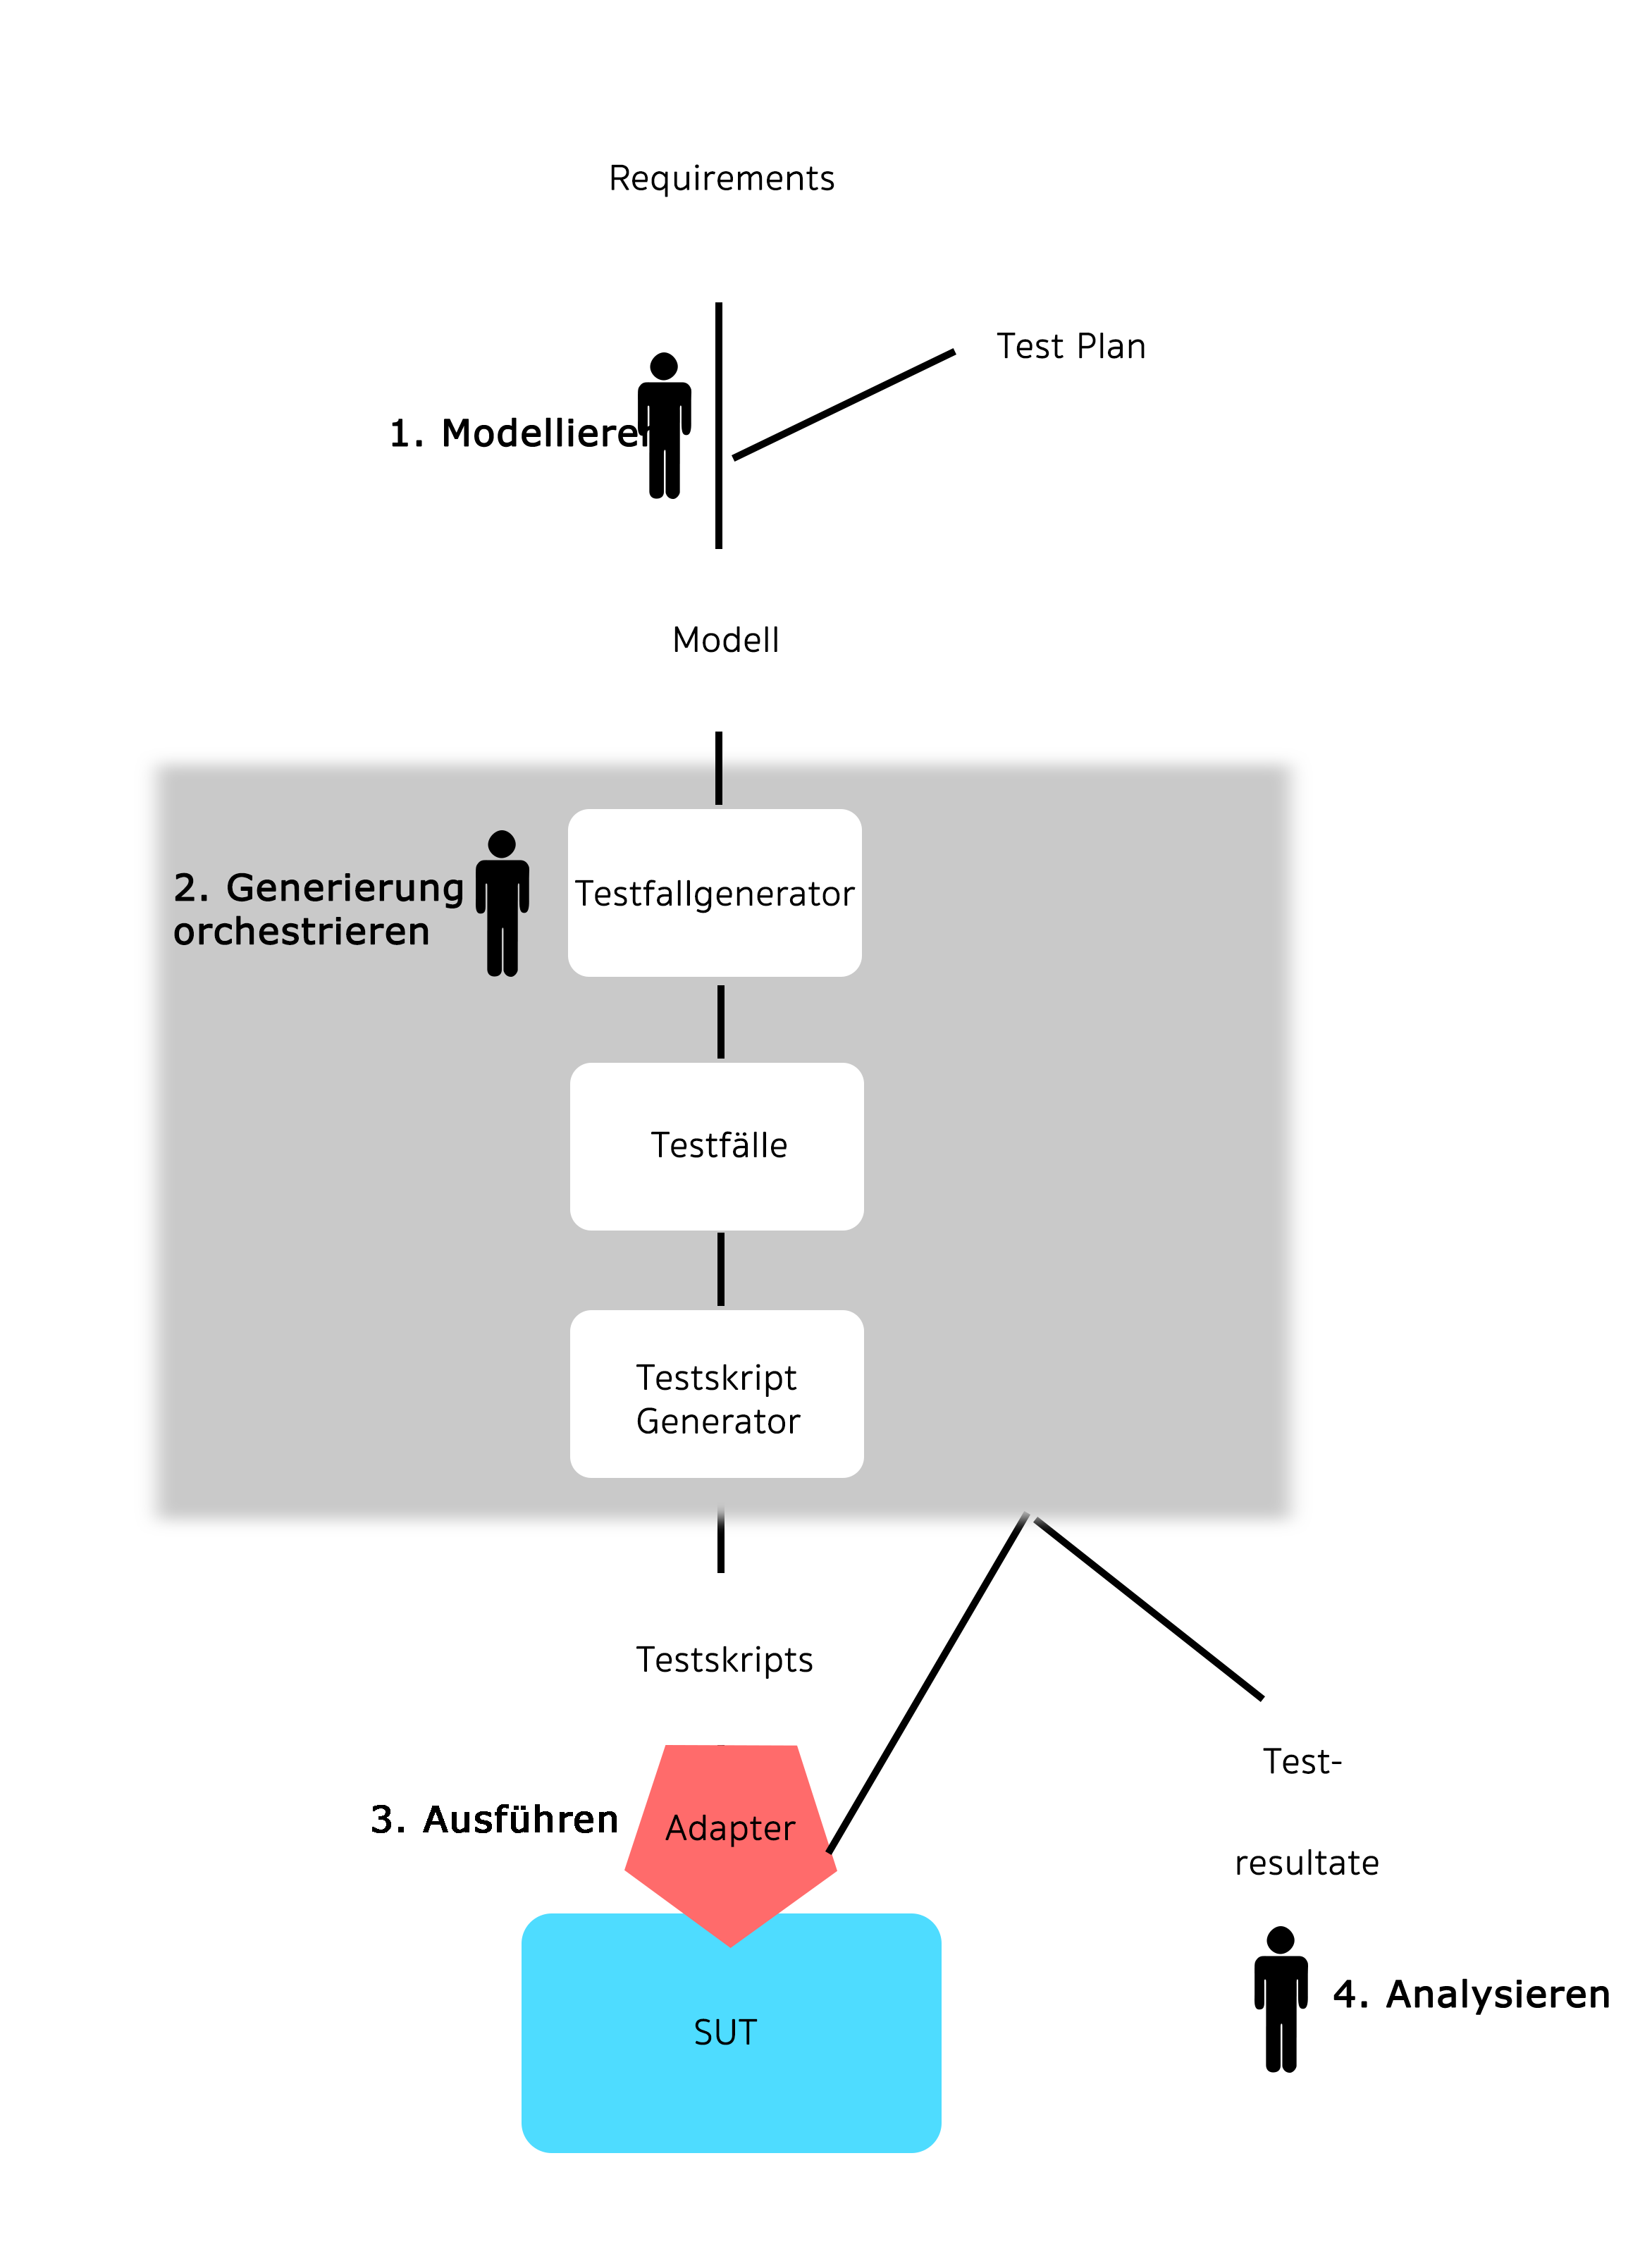
\includegraphics[width=0.9\textwidth]{figures/MBT_Prozess.png}
  \caption{Der MBT Prozess \cite{utting_practical_2007}}
  \label{fig:mbt_prozess}
\end{figure}

Die Schritte 4 und 5 sind Teil jeder Testmethode. Schritt 3 ist Teil einer jeden automatisierten Testmethode. Im Bereich des skritpbasierten Testings wird dieser Schritt von den eingesetzten Tools, so weit wie möglich in den Hintergrund gerückt \todo{Ref zu Skriptbasierten Tests}. Oft gestaltet sich die Übersetzung von abstrakten zu ausführbaren Testfällen aber wesentlich aufwendiger als beworben. (\todo{Irgendeine ref...}).
Die Schritte 1 und 2 unterscheiden MBT also von anderen Testmethoden. Das Modell aus Schritt 1 soll eine abstrakte Darstellung des SUT bzw. seiner Umgebung sein. Das bedeutet es werden nur die, für das Testing relevanten Teile modelliert. Dieses Modell muss demnach viel simpler und kleiner als das reale SUT ausfallen. Außerdem kann es nötig sein, das Modell zu annotieren um informelle Requirements abzubilden, die ansonsten mit der Abstraktion verloren gehen würden. Das Modell sollte nach Fertigstellung verfiziert werden, um formale Korrektheit zu gewährleisten. Dafür bieten viele Modellierungssprachen geeignete Werkzeuge \cite{kaneiwa_consistency_2006}. Außerdem gibt es interaktive Werkzeuge, die das Verhalten eines Modells grafisch darstellen und so das debuggen vereinfachen.\\
Der zweite Schritt, die Generierung von Testfällen aus dem Modell, wird maßgeblich von den gewählten Testauswahlkritereien beeinflusst. Mittels verschiedensten Traversierungsstrategien können aus einem Modell grundsätzlich eine unendliche Menge von Testfällen erzeugt werden \cite{utting_practical_2007}. Die Testauswahlkriterien dienen daher der kontrollierten Einschränkung dieser Menge von Testfällen \todo{Ref. siehe Pfadabdeckung usw}. Der Output dieses Schritts ist also ein Set von abstrakten Testfällen, welche jeweils eine Menge von Operationen definieren die auf dem SUT ausgeführt werden sollen. Da das Modell aber eine vereinfachte Abstraktion des SUT ist, fehlen diesen Operationen die Implementierungsdetails. Diese abstrakten Testfälle sind daher noch nicht ausführbar.\\
Im dritten Schritt werden die abstrakten Testfälle in ausführbare Testskripts verwandelt. An dieser Stelle werden die verschiedensten Ansätze verfolgt. Manche Werkzeuge nehmen als erstes eine Transformation in eine anderen Datenstruktur vor. Das Open Source Werkzeug GraphWalker\footnote{Open Source MBT Tool GraphWalker http://graphwalker.org/} wandelt das Modell erst in einen gerichteten Graphen, bevor aus diesem ein Set von JUnit-Testfällen erzeugt wird. Andere Tools, wie beispielsweise die Implementierung von \cite{pinheiro_model-based_2013}, serialisieren die Modelle erst in ein allgemeineres Format (in diesem Fall XMI\footnote{XML Metadata Interchange Format http://www.omg.org/spec/XMI/}) bevor Testskripts für ein verbreitetes Tool erzeugt werden. Ein Vorteil der sich aus diesem schichtartigen Vorgehen ergibt, ist die Unabhängigkeit von Testplattformen. Solange sich die Logik der Applikation zwischen verschiedenen Plattformen (oder Versionen in anderen Programmiersprachen) nicht unterscheidet, sind die abstrakten Modelle allgemein gültig. Testfälle können so sehr schnell für verschiedenste Plattformen portiert werden.\\
Im vierten Schritt werden die erzeugten Testskripts ausgeführt. Bei der sogenannten \"Online-Execution\" wird der Testfall sofort nach Erzeugung auch ausgeführt. Das Tool, das den Testfall generiert, übernimmt also auch die Ausführung. Im selben Zug muss das Tool auch die Ergebnisse der Ausführung festhalten. Bei der ``Offline'' Erzeugung, wird der Testfall von einem Tool generiert und abgelegt. Anschließend führt ein anderes Werkzeug den Testfall aus und hält dessen Ergebnisse fest. So kann zur Ausführung, Analyse und Historisierung ein gewohntes oder selbst entwickeltes Tool verwendet werden.\\
Im letzten Schritt werden die Ergebnisse der Testfälle analysiert. Auch diesen Schritt teilen sich grundsätzlich alle Testmethoden. Den Detailgrad der Analyse bestimmt größtenteils das Tool, das zur Testausführung verwendet wurde. Dies reicht von einfachen Assertions, wie sie beispielsweise Selenium \footnote{Selenium Browser Automatisierungswerkzeug http://www.seleniumhq.org/} in seinem Grundumfang mitbringt, bis zu sehr detaillierten Berichten inklusive Zeitangaben, Screenshots und kontextuellen Informationen, wie beispielsweise die HP Applikations-Suite UFT \footnote{Testautomatisierungswerkzeug HP Unified Functional Tester http://www8.hp.com/ch/de/software-solutions/unified-functional-testing-automation/} es macht.

\subsection{Vergleich mit klassischem skriptbasierten Tests}
...

\begin{figure}[h] 
  \centering
     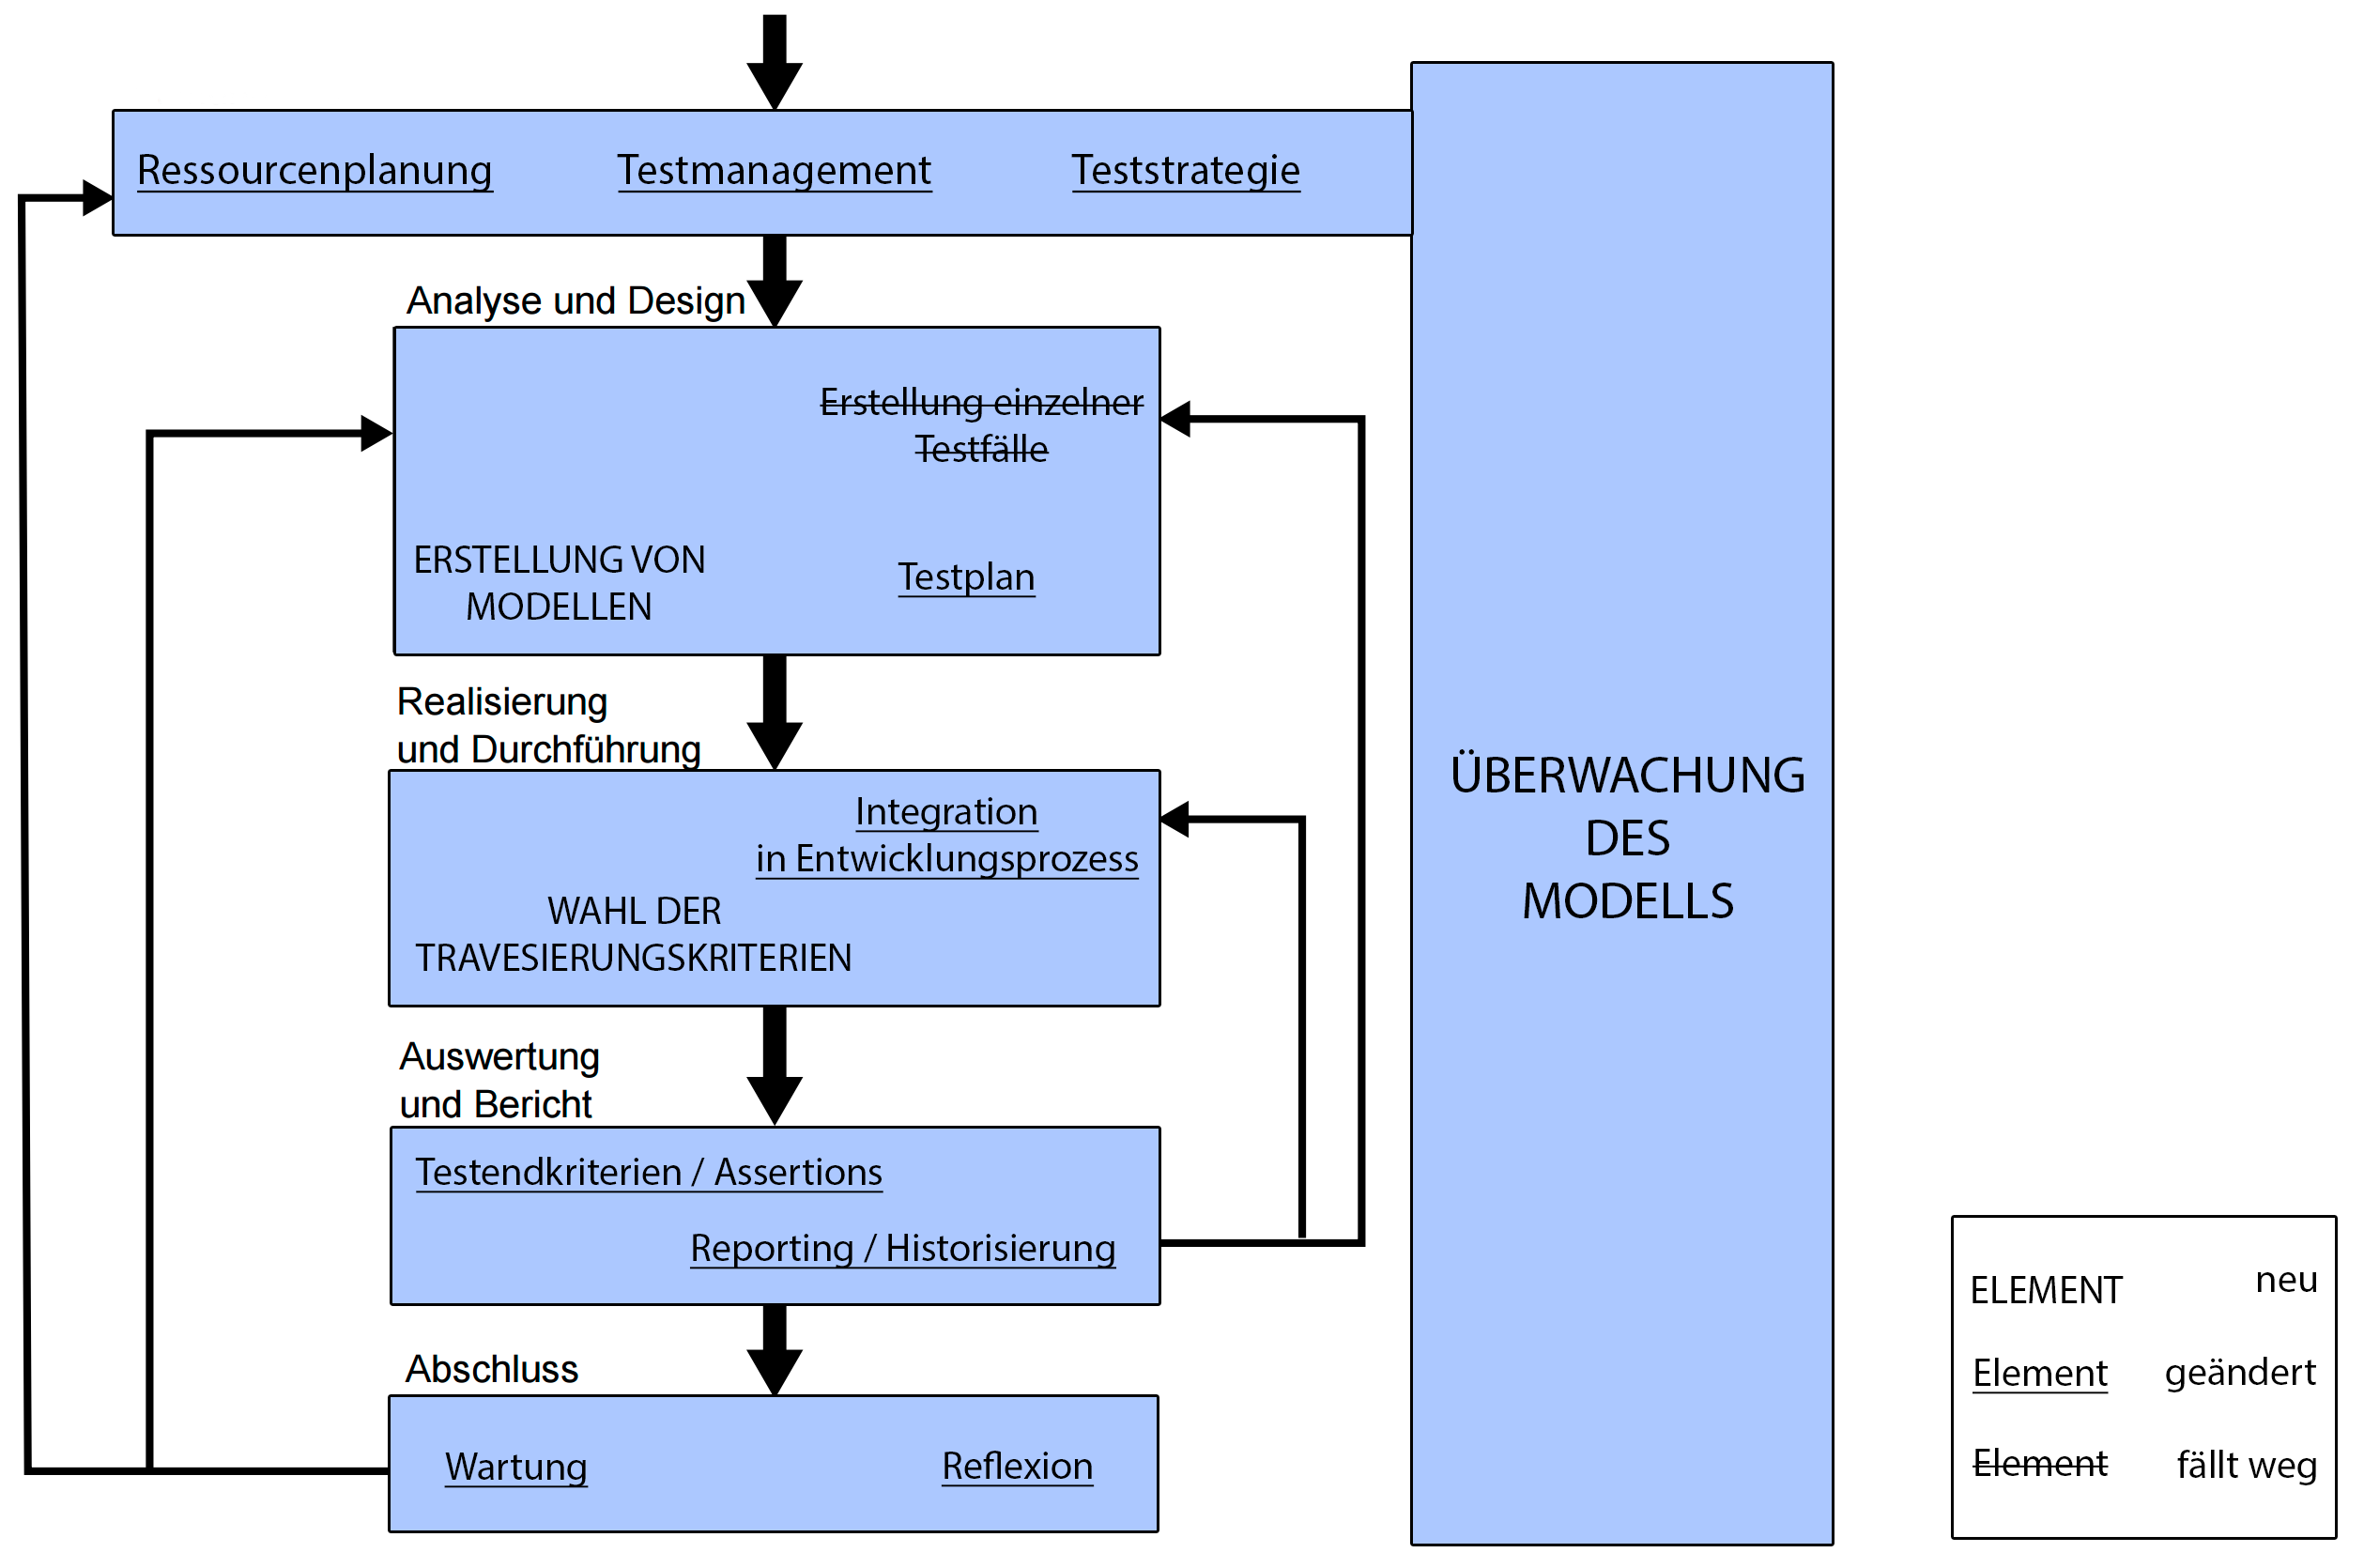
\includegraphics[width=0.7\textwidth]{figures/mbt_vergleich_skript.png}
  \caption{Einordnung von modellbasiertem Testing. Die meisten Aktivitäten im Test-Lifecycle bleiben erhalten, ändern sich aber in der Ausführung. Die Erstellung einzelner Testfälle (scripting) entfällt.}
  \label{fig:fsm_example}
\end{figure}

\subsection{Testauswahlkriterien \& Modellabdeckung}
\label{sec:coverage}

Genau wie auf der Ebene der Unit-Tests, spielt die gewählte Abdeckung eine entscheidende Rolle in modellbasiertem Testen. Verständnis der möglichen Abdeckung und exakte Kenntnisse über das SUT sind der Schlüssel zu einer hochqualitativen Testsuite.\\
Modellabdeckung und Testauswahlkriterien hängen in der Praxis des modellbasierten Testens oft untrennbar zusammen. Wie ein Modell eines Systems vom Ausführenden Programm traversiert wird, entspricht einem genau definierten Testfall in skriptbasiertem Testing. Es hängt vom gewählten Testtool ab ob das Modell, entsprechend der gewählten Abdeckung, immer gleich traversiert wird (so wie das bei den meisten Traversierungsarten von ModelJUnit der Fall ist, siehe Abschnitt \ref{sec:modeljunit}) oder ob bewusst keine immer gleichen skript-artigen Testfälle generiert werden (dieses Konzept der Randomisierung verfolgt Graphwalker, siehe Abschnitt \ref{sec:graphwalker}).\\
Wenn von Abdeckung im MBT-Umfeld gesprochen wird, beziehen sich diese Aussagen immer auf das Modell und damit nur indirekt auf den Quellcode des SUT. Diese Abstraktion ist essentiell, gerade um im agilen Umfeld zeitkritische Qualitätssicherung zu schaffen.\cite{utting_practical_2007} Gleichzeitig muss dieser Umstand Testern und Entwicklern stets bewusst sein. Viele der folgenden Konzepte sind aber abgeleitet von bekannten White-Box Code-Abdeckungskriterien.

\subsubsection{Testauswahlkriterien bei MBT-Tools}
In der Regel werden beim Umgang mit MBT-Tools sogenannte Testauswahlkriterien im Vorfeld der Testgenerierung und Testausführung angegeben. Die Wahl der Testauswahlkriterien beeinflusst also den Algorithmus zur Traversierung des Modells und damit auch die Laufzeit eines Tests.\\
Testauswahlkriterien lassen sich in die folgenden Familien einteilen:

\begin{itemize}
\item \textbf{Strukturelle Abdeckung} sind angelehnt an die Kontrollflussabdeckung, wie sie aus White-Box Tests bekannt ist. Auch Modelle mit Pre- und Postcondition Notation (siehe B-Methode in Abschnitt \ref{sec:bmethod}) werden implizit durch strukturelle Modellabdeckung gesteuert. Auf diese Abdeckungsvarianten wird in den nächsten Abschnitten genauer eingegangen.
\item \textbf{Testdatenabdeckung} beschreibt die Abdeckung anhand von Eingabedaten.
\item \textbf{Requirement-basierte Abdeckung} Kritische Requirements werden vom Tester mit Teilen des Modells verbunden. Bei der Traversierung können nun Requirements vorrangig anvisiert werden.
\item \textbf{Explizite Testfalldefinition} Manche MBT-Tools bieten auch die Möglichkeit explizite Testfälle (also Pfade durch das Modell) zu erstellen.
\end{itemize}

\paragraph{Kontrollflussorientierte Abdeckung}
Die Kontrollflussorientierte Abdeckung gehört zur Familie der strukturellen Abdeckung und hat große Ähnlichkeiten zur Kontrollflussabdeckung im Sinne von Quellcode also White-Box Tests. In Modellnotationen wie OCL oder B-Notation (siehe Abschnitt \ref{sec:bmethod}) lässt sich Kontrollflussorientierte Abdeckung nahezu gleich einsetzen. Der einzige Unterschied ist die Absenz von Schleifen in diesen Modellnotationen, was die Abdeckung weiter einschränkt. Gängige Abdeckungskriterien sind:\cite{rossner_basiswissen_2010}\\
\textbf{Anweisungsüberdeckung} Jede erreichbare Anweisung soll mindestens einmal ausgeführt werden.
\textbf{Zweigüberdeckung} Jedes Konditional im Modell soll von mindestens einem Test einmal positiv traversiert werden und von einem anderen Test mindestens einmal negativ. Zweigüberdeckung setzt Anweisungsüberdeckung voraus.
\textbf{Pfadüberdeckung} Jeder begehbare Pfad durch das Modell muss begangen worden sein.

Zwischen diesen Abdeckungskriterien bestehen Abhängigkeiten. Wenn alle Testsuiten die das Abdeckungskriterium $C_1$ erfüllen, auch das Abdeckungskriterium $C_2$ erfüllen, so ist $C_1$ ein stärkeres Kriterium ($C_1$ subsummiert $C_2$ oder auch $C_1 \longrightarrow C_2$). Allgemein gilt:\\
$ PC \longrightarrow DC \longrightarrow SC $\\
Wobei $PC$ für \textit{Path Coverage} also Pfadabdeckung, $BC$ für \textit{Branch Coverage} also Zweigüberdeckung und $SC$ für \textit{Statement Coverage} also Anweisungsüberdeckung steht.\\
Pfadabdeckung ist in realen Softwaresystemen auf Quellcodeebene nicht erreichbar\cite{utting_practical_2007} weil Schleifen eine potenziell unendliche Menge von verschiedenen Pfaden produzieren könnten. Weil in manchen Modellierungsnotationen (siehe B Notation \ref{sec:bmethod}) aber keine Schleifen modelliert werden können, ist in Pfadabdeckung realistisch erreichbar. Dazu reicht es alle Kombinationen von Zweigüberdeckungsentscheidungen in einer Testsuite zusammenzufassen. Wir gehen hier von einer Bedingung pro Konditional aus. Falls mehrere Bedingungen pro Konditional betrachtet werden sollen, spricht man von \textit{Decision/Condition Coverage}.

\paragraph{Übergangsorientierte Abdeckung}
Auch die übergangsorientierten Abdeckungskriterien gehören zur Familie der Kontrollflussorientierten Abdeckungskriterien. Sie sind aber nicht für Modellnotationen mit Pre- und Postconditions gedacht, sondern für Modelle die von endlichen Automaten abstammen (siehe Abschnitt \ref{sec:fsm}). In diesem Kontext beachtet man nur begehbare Pfade bzw. erreichbare Zustände.\\

\textbf{Zustandsabdeckung} ist gegeben wenn jeder Zustand des Modells mindestens einmal besucht wurde (jedes $e \in Q$ war mindestens einmal gegeben). Es muss nicht zwangsweise jeder Knoten besucht worden sein, da in parallelen Systemen mehrere aktive Zustände auf einem Knoten liegen können.
\textbf{Übergangsabdeckung} ist gegeben wenn jede Zustandsänderung im Modell einmal gemacht wurde.
\textbf{Pfadüberdeckung} Im Kontext der endlichen Automaten spricht man von Pfadabdeckung wenn jeder Pfad vom Startzustand $q_0$ zu einem definierten Endzustand $q_n$ traversiert wurde. Oft macht es aber Sinn nur zyklenfreie Pfade zu betrachten, da sonst unendlich viele Traversierungsarten entstehen. Es gibt weitere Abwandlungen dieses Kriteriums die für jeden Zyklus im Modell mindestens eine Traversierung vorschreiben.

\subsection{Entscheidungshilfe für den Einsatz von MBT}
\label{sec:entscheidungshilfe}
In der Praxis stellt sich für jedes Software-Projektteam die Frage welche Teststrategie am effizientesten, in Bezug auf Qualität und Ressourcennutzung ist. Manuelles Testen gilt in der Industrie immer noch als das am häufigsten eingesetzte Verfahren \cite{guldali_starthilfe_2010}, aber deren Wirksamkeit mindert sich mit steigender Komplexität der zu testenden Software. Skriptbasierte Testautomatisierungstools kommen seit Jahren zum Einsatz. Durch die automatisierte Testausführung, wird der Testprozess schnell und wiederholbar. Verglichen mit manuellen Tests sind skriptbasierte Tests zeitsparender und weniger fehleranfällig. Gleichzeitig müssen skriptbasierte Tests gewartet werden, was einen nicht unerheblichen Ressourcenaufwand bedeuten kann.\\
Als Alternative dazu steht das modellbasierte Testen. Basierend auf \cite{guldali_starthilfe_2010} folgen acht Fragestellungen die zu einer Entscheidung bezüglich der Sinnhaftigkeit des Einsatzes von MBT führen sollen (siehe außerdem Abbildung \ref{fig:entscheidungshilfe_mbt}:

\begin{figure}[h] 
  \centering
     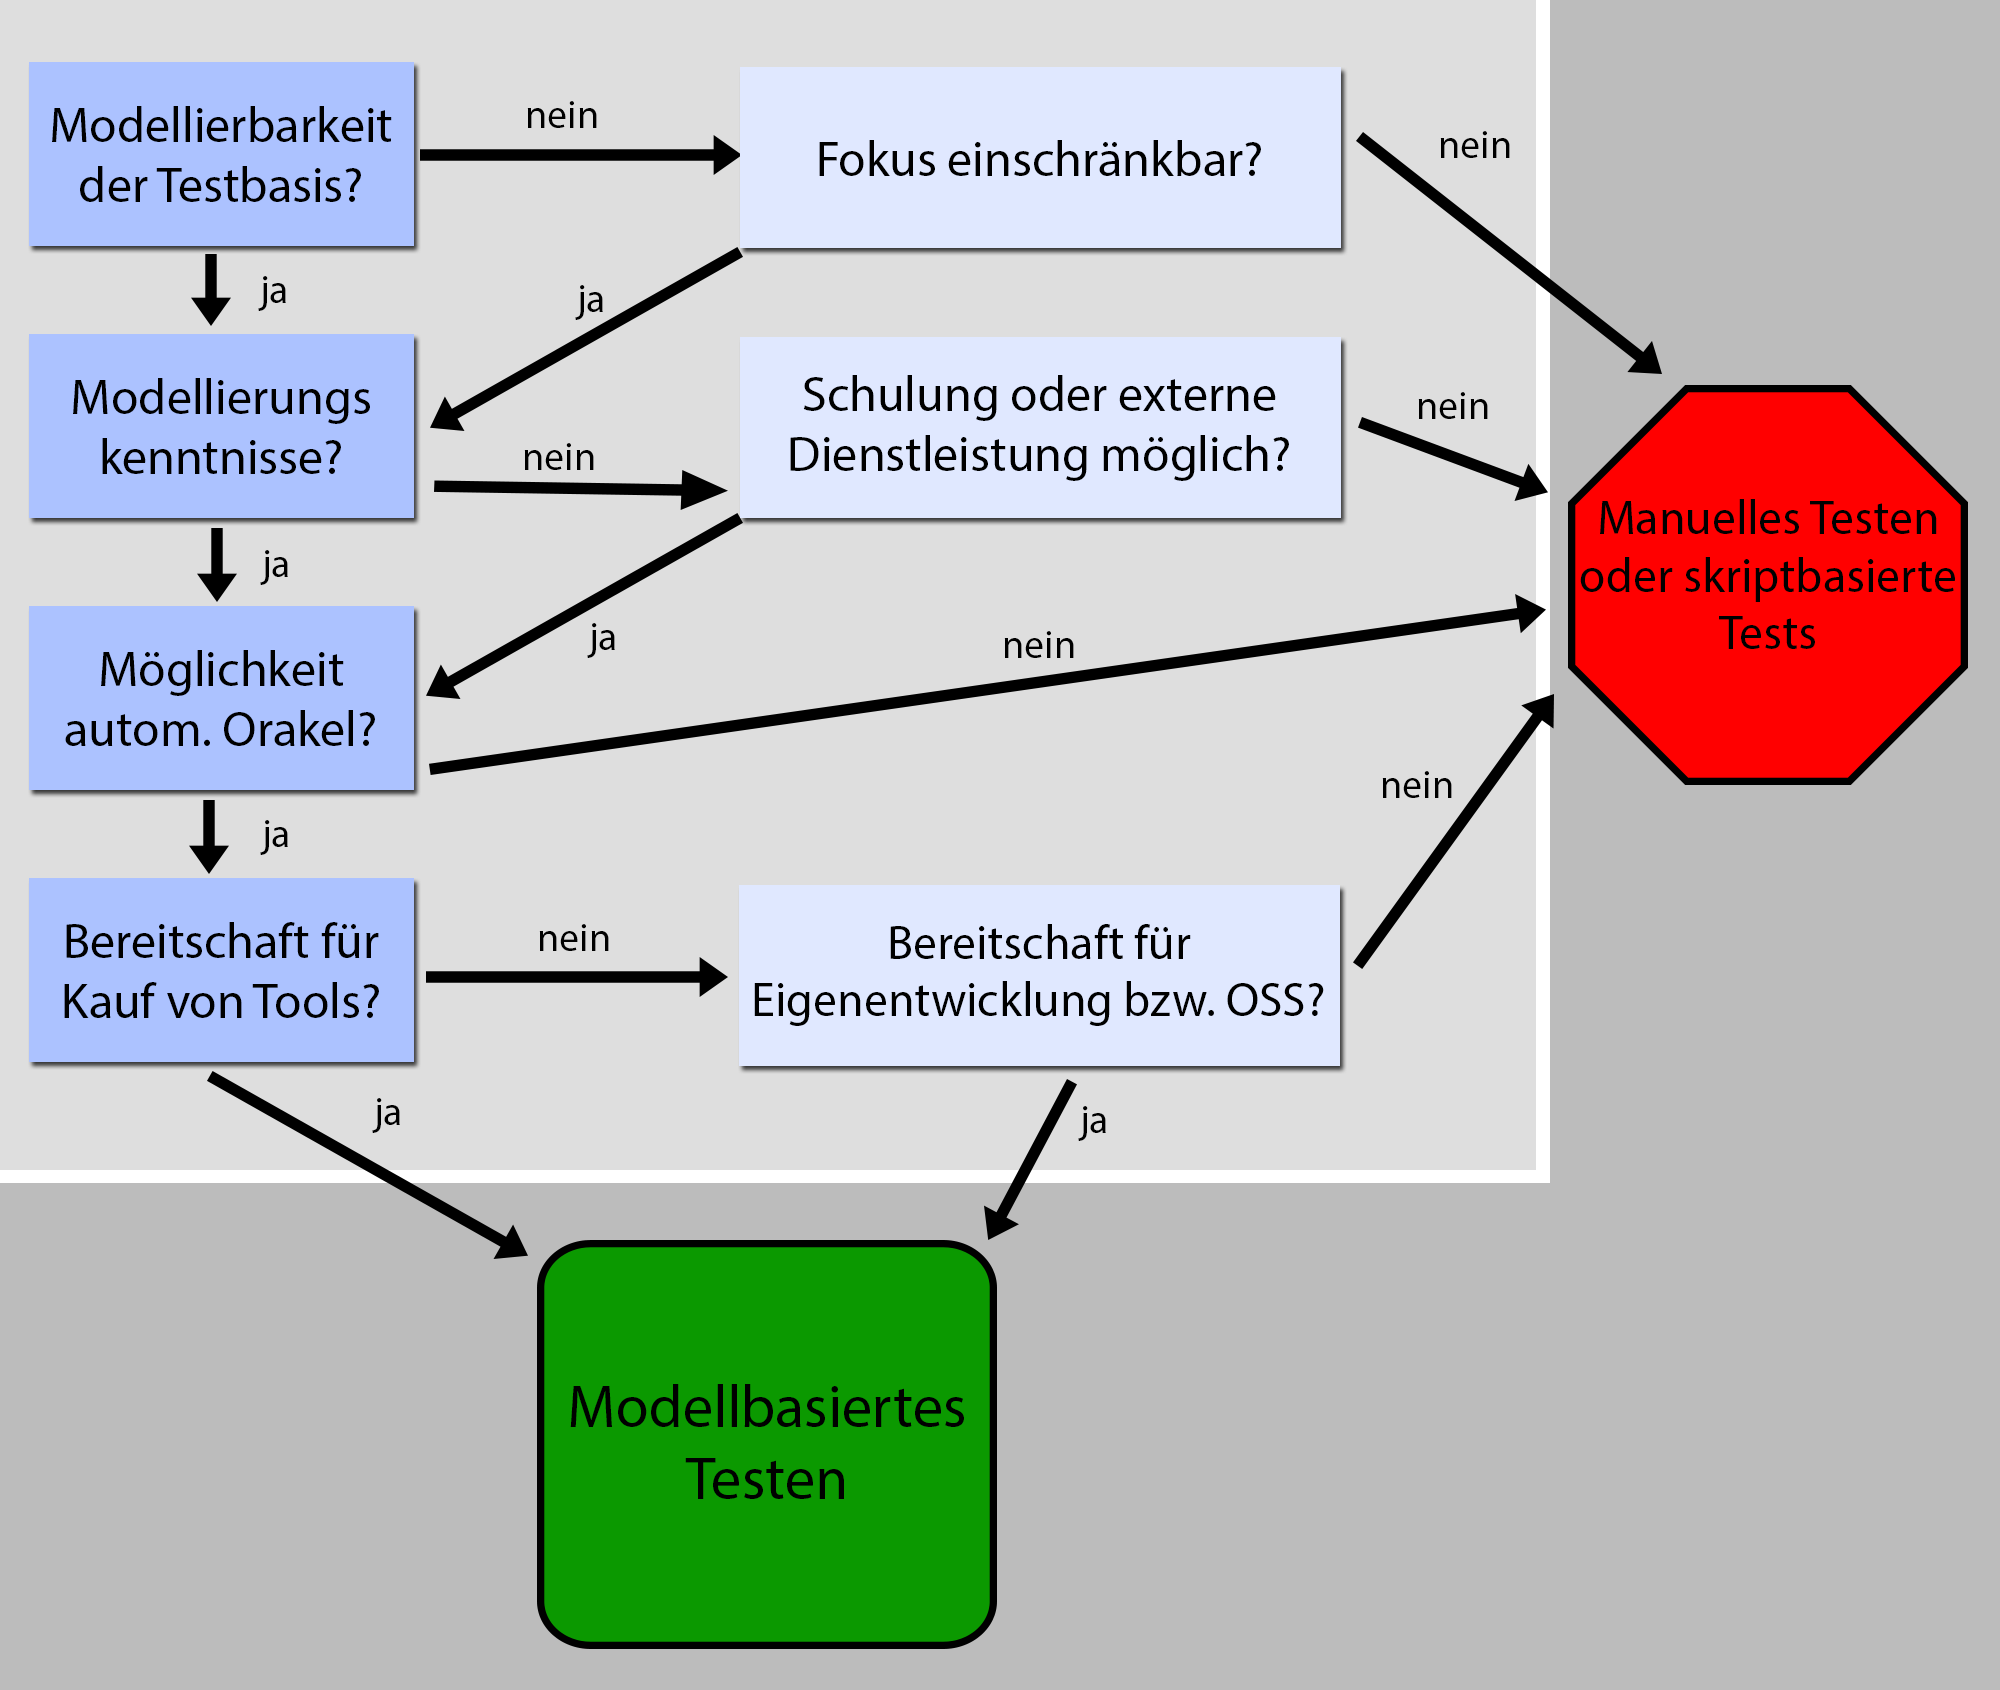
\includegraphics[width=0.9\textwidth]{figures/entscheidungshilfe_mbt.png}
  \caption{Die Zusammenhänge der Entscheidungshilfe für die Einführung von modellbasiertem Testen als Grafik}
  \label{fig:entscheidungshilfe_mbt}
\end{figure}

\begin{itemize}
\item Wie komplex sind die Testbasis und die zu testende Funktionalität?
Die Komplexität des zu testenden Systems ist ein entscheidender Faktor, bei der Auswahl der passenden Teststrategie. Aus niedriger Komplexität oder allgemein wenig Funktionalität, resultieren wenig Testfälle, die mit manuellen Tests durchgeführt werden können. Diese erfordern wenig Planungsaufwand und können schnell ausgewertet werden. Bei steigendem Funktionsumfang kann eine skriptbasierte Ausführung der Testfälle sinnvoll sein. Außerdem kann modellbasiertes Testen die Generierung dieser Testfälle automatisieren.
\item Wie wichtig ist die Überdeckungsanalyse?
Im Software-Testing wird oft anhand der prozentualen Abdeckung des Quellcodes auf die Güte der Teststrategie geschlossen. Mittels skriptbasiertem Testen ist es aber nicht trivial festzustellen, welche Teile des Codes ein Testfall genau abdeckt. Mit MBT lässt sich anhand der Modellüberdeckung schneller feststellen welche Komponenten abgedeckt sind. Außerdem lassen sich Konzepte der Traceability (also der Verfolgbarkeit von Test zu Code) im MBT sehr einfach einführen. Modellbasierte Tests haben daher den nützlichen Nebeneffekt wie ein Vertrag, zwischen Requirement und tatsächlicher Funktionalität, zu funktionieren. Weil modellbasierte Tests oft einfach visuell dargestellt werden können, eignen sie sich auch zu Präsentationszwecken vor Kunden.
\item Wie häufig finden Änderungen in der Spezifikation statt? 
Unzufriedenheit mit skriptbasierten Tests entsteht oft aus teuren Wartungsarbeiten, die nötig werden sobald sich das zu testende System weiterentwickelt. Skriptbasierte Tests können nur zu einem gewissen Grad änderungsunabhängig entwickelt werden. Gerade wenn das Softwareprojekt aus kurzen Entwicklungszyklen besteht (so wie dies bei vielen modernen Projekten der Fall ist), die viel Änderungspotenzial mit sich bringen, sollte MBT in Betracht gezogen werden.
\item Wie wichtig ist die Plattformunabhängigkeit der Testfälle?
Abhängig von der Testebene wo automatisierte Tests auf das System zugreifen, können skriptbasierte Tests nutzlos werden wenn beispielsweise der Austausch einer GUI-Bibliothek erfolgt. Da bei modellbasierten Tests eine strikte Trennung zwischen Testmodell und Adapter zum SUT gemacht wird, muss bei einem Plattformwechsel auch nur dieser Adapter angepasst werden. Auch bei industrieller Software die oft mittels dem Konzept der Software-Familien arbeitet, kann es von Vorteil sein wenn die eigentlichen Testkomponenten unabhängig von der Adapter-Logik bestehen.
\item Ist die Testbasis modellierbar?
Für die Modellierung des SUT ist eine Vielzahl von Notationen verfügbar (siehe Kapitel \ref{sec:notations}). Zustandsbasierte und Ereignisbasierte Notationsarten ermöglich die Modellierung sehr vieler funktionaler Eigenschaften. Wenn sich die Funktionalität der Testbasis aber nur unzureichend modellieren lässt, macht modellbasiertes Testen schlicht keinen Sinn.
\item Hat das Testteam Erfahrung mit Software-Modellierung? / Sind Modellierungskenntnisse im Testteam verfügbar?
Abhängig davon wie die Rollen im Projektteam verteilt sind, muss festgestellt werden ob Modellierungskenntnisse bei denjenigen vorhanden sind, die im weiteren Verlauf Testfälle erstellen und warten. Das Testteam muss deshalb möglicherweise geschult werden. Die Kosten dieser Schulungen, verglichen mit den Aufwänden für manuelles und skriptbasiertes Testen, können entscheidend für die Wahl von MBT sein.
\item Kann das Test-Orakel automatisiert werden?
Da beim modellbasierten Testen, Testfälle in der Regel automatisch generiert werden, sollen auch die erwarteten Testergebnisse modelliert oder in Form von Testdaten hinterlegbar und automatisch prüfbar sein. Falls die erwarteten Systemeigenschaften nicht modellierbar sein können, muss jeder Testfall manuell geprüft werden. Dieser Umstand mindert die Nützlichkeit von modellbasiertem Testen.
\item Ist die Bereitschaft für den Kauf und Einführung eines MBT-Werkzeugs vorhanden?
Eine Einführung von MBT ist immer auch mit Anschaffungskosten verbunden. Auf dem Markt sind verschiedenste Werkzeuge erhältlich \todo{Link zu Marktübersichts Section}. Weiters muss sich das gewählte Tool aber auch in bestehende Umgebungen integrieren lassen (was oft mit weiteren Kosten verbunden ist).
\end{itemize}

\subsubsection{Tool-Landschaft}
Wie auf dem Feld der skriptbasierten Testautomatisierung, ist die Auswahl an Tools zur Unterstützung von modellbasierten Tests vielfältig. Modellbasiertes Testen umfasst in der Regel mehrere Aktivitäten, für die jede Kombination aus passenden kommerziell erhältlichen Werkzeugen herangezogen werden können. Auch die marktführenden Tool-Hersteller haben begonnen ihre Testing Applikations-Suiten für MBT auszurüsten. 

\subsection{MBT Fallstudien}

Model-based Testing von Software wird seit mehr als 20 Jahren aktiv thematisiert, \cite{utting_practical_2007} sei es durch Forschung oder Industrie. Wie in den Leitlinien für den Einsatz von MBT in einem Projekt bereits erwähnt \ref{sec:entscheidungshilfe}, ist ein sinnvoller Einsatz nicht immer gegeben. Diese Leitlinien haben sich unter anderem, durch eben die folgenden Publikation und Fallstudien ergeben, sind aber keineswegs unveränderlich. Durch neue Erkenntnisse im laufenden Einsatz von MBT in den verschiedensten Projekten und durch die stetige Weiterentwicklung der beteiligten Technologien, entwickeln sie sich weiter.\\
Die folgenden Fallstudien geben einen Überblick darüber, wie MBT Methoden in den letzten Jahren eingesetzt wurden.

\paragraph{GUITAR: An innovative tool for automated testing of GUI-driven software \cite{nguyen_guitar:_2014}}Das von den Autoren entwickelte \textit{GUITAR} Framework wurde für modellbasiertes Oberflächentesting entwickelt. Das Werkzeug verhält sich dabei wie eine \textit{Learning Machine}. Soll heißen, es gibt eine endliche Anzahl von diskreten Parametern in das SUT (bedient das Programm) und beobachtet die Ergebnisse (wie sich das SUT verhält). Basierend auf diesen Ergebnisse generiert \textit{GUITAR} automatisch das Modell des SUT. Der Tester kann daraufhin Modifikationen am Modell vornehmen, bevor das eigentliche Testing beginnt.\\ 
In mehreren Fallstudien konnte \textit{GUITAR} Use-Cases nachstellen, in denen die korrekte Bedienung zu unerwarteten Abstürzen des SUT führte. Bedingt durch die geringe Intervention durch den Testentwickler, brachten die Tests eine gewisse Qualitätssteigerung mit wenig Ressourcenaufwand. Diese Methodik kann also hauptsächlich Aussagen über die Stabilität des SUT treffen, lässt aber kaum Schlüsse auf die funktionale Korrektheit zu.\\
Im Hinblick auf Applikationen mit vielen Datenfeldern, oder gar nicht standardisierten Eingabe- und Anzeigefeldern, ist diese Art des Testings nicht hinreichend, weil keinerlei Prüfung auf Korrektheit der angezeigten Daten stattfindet.

\paragraph{Industrial Application of Visual GUI Testing: Lessons learned \cite{alegroth_industrial_2014}}In dieser Publikation aus dem Jahr 2014, erproben Alégroth et al. in zwei groß angelegten Industriefallstudien ein \textit{Visual Testing} Werkzeug. Im Gegensatz zu weitverbreiteten Test-Tools, greift ihr Werkzeug nicht auf Widget-Ebene auf das SUT zu. Bei ihrem Ansatz werden Bitmaps von Oberflächen gemacht (Soll-Zustand) und beim Testdurchlauf mit neuen Bitmaps verglichen (Ist-Zustand). Das Werkzeug lässt feingradige Einstellungen zu, bis zu welchem Grad sich die Bitmaps unterscheiden dürfen um noch als korrekt zu gelten.\\
Die vorgestellte Technik soll manuelles Testen im späten Entwicklungszyklus (Akzeptanz- und Abnahmetests) ergänzen oder sogar ersetzen. Sie hat den Vorteil, dass kaum Aufwand bei der Wartung von Testfällen anfällt und fügt sich gut in eine Continuous Development Umgebung ein. Nachteilig ist aber die Tatsache, dass bei nicht optimaler Konfiguration viele Fehlerfälle (\textit{false negative's}) von Hand geprüft werden müssen.\\
Die Autoren kommen zum Schluss, dass \textit{Visual Testing} sehr wohl seine Daseinsberechtigung in der Qualitätssicherung von komplexer Industriesoftware hat. Sie halten fest, dass die vorgeschlagene Technik in beiden Fallstudien (Applikationen aus dem Bereich Militär und Avionik), genauso effektiv wie manuelle Tests funktioniert. Gleichzeitig ist der Ressourcenaufwand für die Wartung der Testfälle sehr niedrig und die Durchführungsgeschwindigkeit der Testfälle, verglichen mit manuellen Tests, um ein vielfaches höher. Sie halten aber ebenfalls fest, dass \textit{Visual Testing} Werkzeuge schon für den produktiven Einsatz geeignet sind aber noch viel Potenzial zur Verbesserung besteht (sie verwendeten Sikuli \footnote{VGT Test Tool - \url{http://www.sikuli.org/}}).

\paragraph{Microsoft’s Protocol Documentation Program: A Success Story for Model-Based Testing\cite{grieskamp_microsofts_2010}} Diese von Microsoft durchgeführte Fallstudie liefert exakte Zahlen zur Leistung von MBT im Projekt. Bei der Verfikation der Dokumentation von \textit{Client-Server} und \textit{Server-Server} Protokollen hat Microsoft MBT erstmals in einem großen und geschäftskritischen Umfeld eingesetzt. Die Ergebnisse deuten auf ein hohes Ressourceneinsparungspotenzial von MBT hin. Bei der Umsetzung von knapp zehntausend Test- Requirements mit MBT-Methoden ergab sich im Schnitt eine Dauer von 1,39 Personentagen/Requirement. Verglichen mit knapp neuntausend Requirements desselben Projekts, die mit traditionellen Methoden getestet wurden, die durchschnittlich 2,37 Personentage benötigen, ergab sich ein Produktivitätszugewinn von 42\%.

\paragraph{Model-Based Testing and Some Steps towards Test-Based Modelling\cite{tretmans_model-based_2011}} Die Autoren nehmen sich dem Problem Testing aus einem erfahrungsgemäß praxisnahen Blickwinkel an: Die initiale Hürde der Erstellung von Testmodellen, insbesondere auf Basis von schlechter oder nicht existenter Dokumentation. Test-based modelling, also das Generieren von Modellen anhand von bestehenden Testfällen, wird definiert. Für diesen Ansatz setzeen die Autoren \textit{Automata Learning} ein. Dabei handelt es sich um einen \textit{Machine Learning} Ansatz\cite{narendra_learning_1974}. Das Programm 

\subsection{Modellierungssprachen}
\label{sec:notations}
\subsubsection{Endliche Automaten (Finite-State-Machines)}
\label{sec:fsm}
Ein endlicher Automat (oder \textit{finite state machine}) ist eine Form der abstrakten Maschinen. Eine FSM erlaubt die Modellierung des Verhaltens einer Maschine, in diesem Fall eines Computer-Programms.\cite{wagner_modeling_2006}\\
Eine FSM ist immer in genau \textbf{einem} Zustand. Sie besitzt, wie der Name schon sagt, eine endliche Anzahl von Zuständen. Zu jedem Zeitpunkt lässt sich die Maschine genau einem Zustand zuordnen. Zustände enthalten üblicherweise Informationen über die Vergangenheit, also wie die Maschine in den aktuellen Zustand gekommen ist. Diese Informationen müssen aber keineswegs vollständig sein. Aus einem aktuellen Zustand lässt sich nicht notwendigerweise reproduzieren welche Zustände die Maschine zuvor angenommen hat.\\

\paragraph{Aktionen}
Wenn eine FSM ihren Zustand ändert, spricht man von Zustandsübergängen. Weiters kann eine FSM zwischen Aktionen unterscheiden:
\begin{itemize}
\item Eingangsaktion (\textit{entry action}: Aktion wird bei Eintritt in einen Zustand durchgeführt
\item Ausgangsaktion (\textit{exit action}): Aktion wird bei Austritt aus einem Zustand durchgeführt
\item Eingabeaktion (\textit{input action}): Aktion wird basierend auf aktuellen Zustand und einem Eingabewert durchgeführt
\item Übergangsaktion (\textit{transition action}): Aktion wird beim Durchführen eines Übergangs durchgeführt
\end{itemize}

\paragraph{Zustände}
Eine FSM befindet sich zu jedem Zeitpunkt in genau einem Zustand. Mathematisch ist eine FSM folgendermaßen definiert: 

\begin{center}
$FSM := (Q, \Sigma, q_0, \delta, F)$
\end{center}

Wobei $Q$ die endliche Menge an Zuständen ist, $\Sigma$ ein endliches Eingabealphabet und $\delta$ die Übergangsfunktion. Von hoher Wichtigkeit im Kontext der Systemmodellierung sind die Elemente $q_0$ und $F$. Dabei handelt es sich bei $q_0$ um einen klar definierten Startzustand aus der Menge Q und bei $F \subseteq Q$ um eine Menge von Endzuständen. Meistens wird der Startzustand mit einem Pfeil oder einer Farbe gekennzeichnet. Die Endzustände werden meist mit einem doppelten Kreis (siehe Abbildung \ref{fig:fsm_example}) gekennzeichnet.

\begin{figure}[h] 
  \centering
     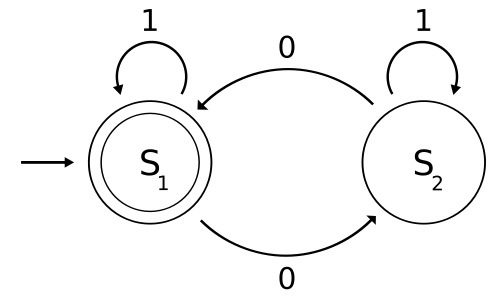
\includegraphics[width=0.5\textwidth]{figures/FSM_example.png}
  \caption{Beispielhafte FSM mit Eingangszustand $S_1$ (gekennzeichnet durch Pfeil von links) der gleichzeitig ein Endzustand ist (doppelter Kreis).}
  \label{fig:fsm_example}
\end{figure}

\subsubsection{B Modelle}
B Notation für abstrakte Maschinen ist eine formale Modellierungssprache zur Beschreibung von Software Systemen.
\begin{itemize}
\item Vor dem Hintergrund eine formale Sprache zu sein, hat B Notation sehr präzise definierte Semantiken.
\item Die Syntax zur Beschreibung von Postconditions ähnelt Code und ist zugänglicher als strikt formaler Annotations-Kalkulus \todo{Footnote zu Annotations-Kalkulus}
\item Im Gegensatz zu strikt formalen Methoden zur Verifikation von Software bietet B einfache Datenstrukturen wie zum Beispiel Sets.
\end{itemize}

B Notation ähnelt den Sprachen die in der Welt der modellgetriebenen Entwicklung verwendet werden, allen voran der Object Constraint Language (OCL).\todo{Footnote zu OCL} 

\paragraph{Die B Methode}
\label{sec:bmethod}
Bei Verwendung der B Methode wird die Korrektheit eines Software Systems, ausgehend von einem abstrakten Modell, bewiesen. Zugrunde liegt die, weiter oben erläuterte, B Notation.\\
In der kompletten B Methode wird ein abstraktes Modell schrittweise verfeinert. Parallel verifizieren Tools automatisch ob tatsächlich eine korrekte und detailliertere Version des Modells erstellt wurde. Nach mehreren Iterationen generieren erhältliche Tools eine meist sehr große Anzahl an mathematischen Implikationen. Nach rigorosen Beweisen all dieser Implikationen kann das System, so wie es modelliert wurde, als korrekt angesehen werden.\\
Im Gegensatz zur kompletten B Methode wird die B Notation oft viel leichtgewichtiger verwendet. Utting und Legeard\cite{utting_practical_2007} schlagen einen Ansatz vor, bei dem nur ein kleiner, für den Test relevanter, Teil des SUT modelliert wird. Außerdem werden nicht mehrere Iterationen zur Verfeinerung des Modells gemacht sondern nur eine. Aus diesem Modell werden automatisch Testfälle generiert, die die Unterschiede zwischen Modell und tatsächlicher Implementation offenbaren. Wie bei allen MBT-Methoden muss anschließend aber trotzdem vom Tester manuell festgestellt werden, ob es sich tatsächlich um ein Fehlverhalten handelt oder ob ein Fehler bei der Modellierung passiert ist.\\
Dieser Ansatz garantiert keine Korrektheit des Systems, wie es die komplette B-Methode macht, ist aber viel praxistauglicher. Die B-Methode wird verwendet um sehr sicherheitskritische Systeme zu testen, die über einen langen Zeitraum keiner Weiterentwicklung ausgesetzt sind. Bei Systemen mit diesen Eigenschaften lassen sich die hohen Aufwände rechtfertigen und stellen einen klaren Mehrwert dar. Ein bekanntes Beispiel für die erfolgreiche Anwendung der B-Methode findet sich in Frankreich, wo Teile des Pariser U-Bahn Systems mit der B-Methode verifiziert wurden. \cite{lecomte_formal_2007}

\paragraph{Beispielhafte Anwendung der leichtgewichtigen B-Methode}
Am Beispiel eines Getränkeautomaten sollen die Grundzüge der B-Notation erläutert werden. Um das Beispiel kurz zu halten und um aufzuzeigen, dass ein Modell nur einen Teil des SUT repräsentieren kann, soll der gezeigte Automat nur Münzen aufnehmen können (und den Betrag der eingeworfenen Münzen anzeigen) und wieder auswerfen können. Außerdem besitzt der Automat ein Limit, bei dessen Erreichen alle zuvor eingeworfenen Münzen wieder ausgeworfen werden.

\begin{lstlisting}[caption={Modell eines Getränkeautomaten in B-Notation},label=lst:b-notation]
MACHINE
	GET_AUTOMAT
VARIABLES
	balance, limit
INVARIANT
	limit : INT & balance : INT &
	0 <= balance & balance <= limit
INITIALISATION
	balance := 0 || limit := 200
OPERATIONS
	reject <-- insertCoin(coin) =
		PRE coin : { 5, 10, 20, 50, 100 }
		THEN
		IF coin + balance <= limit
		THEN
			balance := balance + coin || reject := 0
		ELSE
			reject := coin
		END
	END
	money <-- returnButton = money := balance || balance := 0
END
\end{lstlisting}

Es ist zu erkennen, dass B-Notation eine sehr lesbare Notation besitzt. Die Syntax \textit{out <-- name(in)=...} beschreibt eine Prozedur mit einem Rückgabewert (\textit{out}) und einem Eingabewert (\textit{in}). Die Sektion \textit{INVARIANT} beschreibt Invarianten, also Werte bzw. Aussagen im Programm die sich während der gesamten Laufzeit nicht ändern (equivalent zu Invarianten bei der Verfikation mit formalen Methoden). Der doppelte senkrechte Strich soll kein logischer Operator sein, sondern eine undefinierte Komposition. Die Verkettung von mehreren Operationen mittels diesem Operator soll bedeuten, dass es keinen Unterschied macht in welcher Reihenfolge die Operationen ausgeführt werden. Das folgende Beispiel veranschaulicht diesen Unterschied.\\

Die folgenden beiden Zeilen sind equivalent zueinander.
\begin{verbatim}
money := balance || balance := 0
balance := 0 || money := balance
\end{verbatim}

Bei klassischer sequentieller Komposition, also Hintereinanderausführung, sind die folgenden beiden Zeilen aber keineswegs equivalent.
\begin{verbatim}
balance := 0;
money := balance;
\end{verbatim}

Aus diesem sehr einfachen und abstrakten Modell könnte ein Tool zum Beispiel die folgenden Testfälle generieren:\\


\begin{verbatim}
Test1: init:
	returnButton = 0
	insertCoin(5) = 0
	returnButton = 5
\end{verbatim}

\begin{verbatim}
Test2: init:
	insertCoin(100) = 0
	insertCoin(100) = 0
	insertCoin(5) = 5
\end{verbatim}

Die beiden Testfälle gehen von einem Limit von 200 Einheiten aus. Solaneg die eingeworfene Menge plus der Saldo unter dem Limit bleiben, wird nichts ausgeworfen. Jeder Betrag darüber wird sofort retourniert (siehe letzte Zeile in Testfall 2). In Klammer stehen also die Eingabewerte (entsprechend \textit{in} im Modell) und die Werte rechts vom Gleichheitszeichen stellen die erwarteten Ausgabewerte dar (entsprechend \textit{out} im Modell).\\
Die hier gezeigte Syntax entspricht der ASCII B Notation, welche auch von den meisten Werkzeugen verwendet wird\footnote{Das Tool ProB der Heinrich-Heine-Universität, welches auch zur grafischen Darstellung und Animation von Modellen verwendet werden kann, kann ebenfalls mit ASCII B benutzt werden. \url{http://stups.hhu.de/ProB/}}.\\

Modelle in B Notation können folgende Dimensionen definieren (von denen einige bereits in \ref{lst:b-notation} zu sehen sind).

\begin{itemize}
\item \textit{MACHINE} ist ein Bezeichner mit dem auf das Modell Bezug genommen werden kann.
\item \textit{SETS} definiert enumerierte Datentypen.
\item \textit{CONSTANTS} definiert konstante Werte die sich zur Laufzeit nicht verändern.
\item \textit{PROPERTIES} weist den zuvor deklarierten Konstanten Werte zu.
\item \textit{VARIABLES} deklariert Variablen.
\item \textit{INVARIANT} definiert welche Wertbereiche die Variablen haben und welche Abhängigkeiten zwischen den Variablen bestehen.
\item \textit{INITIALISATION} eine Menge von \textit{parallelen} Zuweisungen zum Zweck der initialen Belegung der Variablen.
\item \textit{OPERATIONS} definiert alle möglichen Operationen bzw. Prozeduren die innerhalb des Modells aufgerufen werden können. Es können rein lesende Operationen als auch Operationen mit Lese- und Schreibzugriff definiert werden. Außerdem sind Konditional-Konstrukte, wie der If-Block in \ref{lst:b-notation}, zulässig. Um die Korrektheit einer Operation einfacher zu überprüfen ist es nicht erlaubt eine Variable mehrfach zu beschreiben. Außerdem gibt es keine Schleifen, da diese die Verfikation um ein vielfaches erschweren würden.
\end{itemize}
\todo{Weiter mit Utting 85...}
\subsubsection{UML/ UML Testing Profile}
\paragraph{Test-Driven Testing mit UTP}
Businessapplikationen (unter anderem in den Bereichen Finanz-, Versicherungs- und Gesundheitswesen) basieren auf großen Datenbeständen. Diese wurden oft über Jahre und Jahrzehnte gesammelt und gespeichert. Zwischen den Datensätzen bestehen Abhängigkeit, die das Verhalten der Applikation stark beeinflussen. Solche Systeme werden als \textit{datengetrieben (data-driven)} bezeichnet. Das Testing von solchen Systemen ist dementsprechend gekennzeichnet durch die Verwendung von vielen, oft relationalen, Datensätzen. Die Praxis zeigt, dass sich die Datenstrukturen innerhalb eines Systems ändern und von der ursprünglichen Spezifikation abdriften. Es ist also von höchster Wichtigkeit, das Testdatenmangement angemessen zu designen um hohe Wartungsaufwände zu minimieren.\cite{baker_model-driven_2005}\\
Das UML Testing Profile bietet Unterstützung von datengetriebenen Tests in mehreren Formen.

\subparagraph{Wildcards in Ausprägungsspezifikationen}
UTP bietet vereinfachte Wildcards um zu spezifizieren, dass ein Attribut einen beliebigen Wert annehmen darf (annotiert mit \textit{?}) oder sogar keinen Wert haben darf (annotiert mit \textit{*}). Diese Wildcards können in sogenannten Ausprägungsspezifikationen (\textit{Instance Specifications} \footnote{Ausprägungsspezifikationen wurden im UML 2 Standard definiert \url{http://www.omg.org/spec/UML/2.4/} }) eingesetzt werden. Mit diesen kann die Existenz einer Entität innerhalb des modellierten Systems beschrieben werden. Instanzspezifikationen müssen ausdrücklich nicht vollständig sein, was dem Testfalldesigner zugute kommte, da oft nur wenige Attribute von Bedeutung sind. Solche Ausprägungsspezifikationen erlauben, die Definition von Testdaten ohne sie in Sequenzdiagramme `hart' zu codieren.

\begin{figure}[h] 
  \centering
     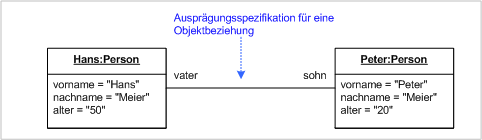
\includegraphics[width=0.7\textwidth]{figures/uml_instance.png}
  \caption{Eine UML Ausprägungsspezifikation. Sowohl eine Instanz der Klasse als auch eine Relation kann als Ausprägung dargestellt werden. (German Wikipedia user Gubaer [GFDL (http://www.gnu.org/copyleft/fdl.html) or CC-BY-SA-3.0 (http://creativecommons.org/licenses/by-sa/3.0/)], via Wikimedia Commons)}
  \label{fig:uml_instance}
\end{figure}